\chapter{Evaluation and Discussion}
\label{ch:evaluation}

In this chapter we go through a few case studies and discuss the difference
between the specification translations if any. Table \ref{tab:specstranslated}
shows the specifications we have translated into Isabelle using \gls{zmath}. We
have classified these examples to show the different types of specifications
which can be translated using the \gls{zmath} tool-kit. In this chapter we take
one example from each class (Steamboiler from appendix \ref{app:steamboiler}, ModuleReg from chapter \ref{ch:fullexample}
 and AutoPilot from appendix \ref{app:semiform}) 
and describe in more detail how the translation was done.

\begin{table}[H]
\begin{tabular}{|l|l|}
\hline
\textbf{Examples using only terms} & \textbf{Examples using sets and terms} \\
\hline
Vending Machine & Birthday Book \\
SteamBoiler & ClubState \\
\cline{1-1}
\cline{1-1}
\textbf{Incomplete translations} & Clubstate2 \\
\cline{1-1}
Autopilot & GenDB \\
A specification which fails ZCGa & ModuleReg \\
A specification which fails ZDRa & ProjectAlloc \\
& Timetable \\
& Videoshop \\
& TelephoneDirectory \\
& ZCGa \\
\hline
\end{tabular}
\caption{A table showing the specifications we have translated into Isabelle using \gls{zmath} \label{tab:specstranslated}}
\end{table}

We have categorised the specification into three groups; specifications which
only use terms, specifications which use both terms and set and specifications
which the translation is incomplete for a variety of reasons.
These categories are important as the examples using sets and terms are more complex
then the specifications only using terms. This is because there is an extra ZCGa type
to manage. The specification which are categorised as "incomplete" can be using terms
and sets however they are not full specification so have not been fully translated into 
Isabelle and/or have proofs to check the stateInvariants.
All the
specifications we have translated are `state based specifications', which means
they operate within a state and to change the state their may become
precondition and postconditions within the state. Some specifications are
described differently such as functional specifications, however 
it was difficult to find full examples of functional specification and therefore
we couldn't add it to the list of examples.

\section{Complexity of specifications}

This section we analyse the complexity of the specifications we have translate
using \gls{zmath}. First we check the complexity of the raw \LaTeX{}
specification file, without any annotation. Then we discuss the complexity of
the \gls{zcga} annotated specifications and \gls{zdra} annotated specifications
and how this affects the translation into Isabelle.

\subsection{Raw Latex Count}

Table \ref{ch:evaluation} shows how long each specification is by amount of lines of
code and environments uses. We have listed the specifications in decreasing
complexity of how many lines of \LaTeX{} the raw specification has.

\begin{table}[H]
\centering
\begin{tabular}{|l |l | l |l |l|| l|}
\hline
\textbf{Specification} & \multicolumn{4}{l||}{\textbf{Environment}} &
\textbf{Lines of \LaTeX} \\
\cline{2-5}
& Zed & Schema & Axdef & \textbf{Total} & \\
\hline
Steamboiler & 10 & 34 & 3 & 47 & 507 \\
ProjectAlloc & 4 & 17 & 0 & 21 & 213 \\
VideoShop & 3 & 15 & 0 & 18 & 166 \\
TelephoneDirectory & 6 & 11 & 0 & 17& 133 \\
ClubState & 4 & 11 & 1 & 16 &129 \\
ZCGa & 2 & 9 & 0 & 11 & 128 \\
GenDB & 2 & 7 & 0 & 9 & 114 \\
Timetable & 1 & 6 & 1 & 8 & 92 \\
BirthdayBook & 3 & 7 & 0 & 10 & 83 \\
AutoPilot & 2 & 3 & 0 & 5 & 83 \\
ClubState2 & 1 & 6 & 1 & 8 & 80 \\
Vending Machine & 4 & 7 & 0 & 11 & 68 \\
ModuleReg & 1 & 3 & 0 & 4 & 43 \\
\hline
\end{tabular}
\caption{How many zed, schema and axdef environments and lines of \LaTeX{} code makes up each specification \label{tab:numbersspec}}
\end{table}

We list information about how many different environments and lines of \LaTeX{}
make up each specification in table \ref{tab:numbersspec}. The environment
numbers count how many different types of environments exist within the
specification. That is how many `\verb|\begin{schema}...\end{schema}|' or
`\verb|\begin{zed}|... etc. We add up the total amount of environments in the
specification. From the table we can see that for most of the specifications the
more lines of \LaTeX{} there is then the total amount of environments increase.
However, there are three exceptions to this trend. The `\emph{BirthdayBook}'
specification, `\emph{ClubState2}' specification and `\emph{Vending Machine}'
specification. Specifications for systems are can always be written in a variety
of ways and still have the same meaning. Even formal specifications can be
written different ways. For example one may have the following declarations:

\begin{zed}
t:\nat \\
l: \nat 
\end{zed}

However, this declaration can also be written as the following:
\begin{zed}
t,l: ;\nat
\end{zed}

Thus removing a line. Formal specifications can also include comments written in
natural language which are not part of the formal script. These extra comments
about the specification may have also added to the line count in table
\ref{tab:numbersspec}.

However, there are also many lines which can not be simplified in the specification
for example if a specification uses a certain Z-type i.e. `\texttt{COLOUR}' then
`\texttt{COLOUR}' must be declared at the beginning of the specification:
\verb|[COLOUR]|\\
in the specification this line can not be removed. Therefore
we use the number of lines plus the number of environment to discuss the complexity.

The number of environments is also used to discuss complexity as we could have simple
program which only has one function (such as a program which outputs a number). This 
type of specification would only have 1 output schema and therefore be considered as 
quite simple. Other programs/specifications can have many different functions and 
therefore many different environments. Hence, when we discuss complexity in this chapter
the more the environments a specification has the more complex it is.

\subsection{ZCGa Count}

In this section, we evaluate the \gls{zcga} annotations on the specifications.
We describe how many of each \gls{zcga} annotations occurs for each
specification we have translated.

\begin{table}[H]
\centering
\begin{tabular}{|l |l | l |l | l| l | l |}
\hline
\textbf{Specification} & \multicolumn{6}{c|}{\textbf{ZCGa WeakTypes}}\\
\cline{2-7}
 & \cgatext{} & \declaration{} & \expression{} & \term{} & \set{} &
 \definition{} \\
\hline
Steamboiler & 297 & 26 & 282 & 595 & 4 & 0 \\
ProjectAlloc & 98 & 43 & 113 & 154 & 165 & 0\\
VideoShop  & 87 & 31 & 75 & 119 & 95 & 0 \\
TelephoneDirectory & 78 & 26 & 53 & 72 & 50 & 0 \\
ClubState & 75 & 17 & 51 & 55 & 51 & 0 \\
ZCGa & 73 & 27 & 67 & 35 & 133 & 0 \\
GenDB & 45 & 24 & 71 & 117 & 121 & 1 \\
Timetable & 35 & 15 & 53 & 48 & 114 & 0 \\
BirthdayBook & 26 & 11 & 24 & 28 & 19 & 0 \\
AutoPilot & 16 & 9 & 19 & 31 & 2 & 0\\
ClubState2 & 34 & 7 & 37 & 22 & 72 & 0 \\
Vending Machine & 16 & 7 & 21 & 37 & 0 & 0 \\
ModuleReg & 20 & 6 & 18 & 13 & 31 & 0 \\
\hline
\end{tabular}
\caption{How many of each grammatical category exists in each specification. \label{tab:specgram}}
\end{table}

The amount of times a \gls{zcga} weak type occurs in each specification is shown
in table \ref{tab:specgram}. We remind the reader the colours corresponding to
each grammatical type are: \cgatext{schematext}, \declaration{declaration},
\expression{expression}, \term{term}, \set{set} and \definition{definition}. In
this instance we don't use \specification{specification} as we assume each
document contains a single specification.

In our sample set we only have one specification (GenDB) with a
`\texttt{definition}' annotation. This \texttt{definition} is locally defined
within the specification. The `\emph{Vending Machine}' specification only uses
\texttt{terms} and therefore there are no \gls{zcga} \texttt{term} annotations.
However the `\emph{StemBoiler}' specification also only uses term yet there are
4 \texttt{set} \gls{zcga} annotations. This is because some of the
\texttt{terms} used in the specification have to be introduced by a \texttt{set}.
For example in the \emph{SteamBoiler} specification we have the following
annotation:

\begin{verbatim}
\begin{zed}
\set{State} ::= \term{init} | \term{norm} |
\term{broken} | \term{stop}
\end{zed}
\end{verbatim}

Although the set \verb|State| is annotated as a set, it is not used in any of
the schema's in the rest of the specification. It is only defined to present the
terms \verb|init|, \verb|norm|, \verb|broken| and \verb|stop| which are used in
the specification.

We expect there to be more \texttt{schemaText}'s then \texttt{declarations} and
\texttt{expressions} combined as \texttt{schemaText} contains all
\texttt{declarations}, \texttt{expressions} and SchemaNames however, from the
table we can see that this is not always the case. For example in the
\emph{ProjectAlloc} example, there are 98 \texttt{schemaText}, 43
\texttt{declarations} and 113 \texttt{expressions}. The reason for this could be
because a single \texttt{expression} can in itself contain many
\texttt{expressions}. For example the following \texttt{schemaText} has been
taken from the \emph{ProjectAlloc} specification:

\begin{verbatim}
\text{\expression{\forall 
\declaration{\term{lec}: \expression{\dom maxPlaces}}\\
@ \expression{\term{\# (\set{\set{allocation}
\rres \set{\{\term{lec}\}}})} \leq \term{\set{maxPlaces}~\term{lec}}}}}
\end{verbatim}

In this example we can see that there contains 1 annotated \texttt{schemaText}
but 3 \texttt{expressions}. Another reason why there may be more
\texttt{expressions} than \texttt{schemaText} is because when annotating a
specification with \gls{zcga}, \texttt{declarations} also contain
\texttt{expressions}. If we have the following example, again taken from the
ProjectAlloc specification:

\begin{verbatim}
\text{\declaration{\set{studInterests}, \set{lecInterests}:
\expression{PERSON \pfun\iseq TOPIC}}}
\end{verbatim}

The \gls{zcga} text contains 1 annotation of \texttt{SchemaText}, 1 annotation
of a \texttt{declaration}, 2 annotations of \texttt{sets} and 1 annotation of an
\texttt{expression}. Since this is the case we expect to see more expressions
than declarations in every specification, which is true according to table
\ref{tab:specgram}.

The SteamBoiler specification has by far the most ZCGa weak types in total at 1204.
Therefore in terms of complexity it would take the longest to annotate in ZCGa.
In terms of doing a ZCGa weak type check it would also take the longest as the ZCGa
would have to parse through all 1204 weak types and check they are correct.
There are only 4 `\texttt{sets}' in the SteamBoiler specification but in our case
this doesn't make a difference because the ZCGa weak typing rules are similar for set
and term. Therefore if the next complex specification (ProjectAlloc) still wouldn't class
as being more complex than the Steamboiler specification. 
GenDB can also be argued as being complex as it contains the highest amount of weak types
 \textbf{and} containing a definition. However as the specification only contains 1 
 definition out of a total of 378 weak types, we can not dispute that GenDB has a strong
 case for being the most complex. This conclusion is drawn just by analysing 
the amount of ZCGa weak types. We will look at ZDRa in the next section.

\subsection{ZDRa Count}

In this section we analyse the amount of \gls{zdra} instances and relations are
labeled for each of the specifications we translated. We give details of the
amount of instances in table \ref{tab:speczdracount} and give details of the
amount of relations in each specification in table
\ref{tab:speczdrarelationscount}.

\begin{table}[H]
\centering
\begin{tabular}{|l |l | l |l | l| l | l | l | l | l | l |}
\hline
\textbf{Specification} & \multicolumn{10}{c|}{\textbf{ZDRa Instances}}\\
\cline{2-11}
 & \textbf{A} & \textbf{SS} & \textbf{IS} & \textbf{CS} & \textbf{OS} &
 \textbf{TS} & \textbf{PRE} & \textbf{PO} & \textbf{O} & \textbf{SI}  \\
\hline
Steamboiler & 6 & 2 & 2 & 21 & 6 & 6 & 21 & 23 & 12 & 1  \\
ProjectAlloc & 0 & 1 & 1 & 5 & 11 & 0 & 11 & 6 & 22 & 1 \\
VideoShop &  0 & 1 & 1 & 3 & 10 & 0 & 13 & 4 & 20 & 1  \\
TelephoneDirectory & 0 & 1 & 1 & 4 & 5 & 5 & 8 & 5 & 10 & 1 \\
ClubState & 1 & 1 & 1 & 4 & 6 & 4 & 9 & 6 & 11 & 0 \\
ZCGa & 0 & 1 & 1 & 6 & 1 & 0 & 6 & 7 & 2 & 1 \\
GenDB & 0 & 1 & 1 & 4 & 2 & 0 & 6 & 5 & 4 & 1 \\
Timetable & 1 & 1 & 1 & 4 & 0 & 0 & 4 & 5 & 0 & 1 \\
BirthdayBook & 0 & 1 & 1 & 1 & 4 & 2 & 4 & 2 & 8 & 1 \\
AutoPilot & 0 & 2 & 0 & 1 & 1 & 0 & 1 & 1 & 2 & 0 \\
ClubState2 & 1 & 2 & 1 & 3 & 0 & 0 & 3 & 4 & 0 & 2 \\
Vending Machine & 0 & 1 & 0 & 3 & 0 & 3 & 3 & 2 & 0 & 0 \\
ModuleReg & 0 & 1 & 0 & 2 & 0 & 0 & 2 & 2 & 0 & 1 \\
\hline
\end{tabular}
\caption{How many of each ZDRa instances exists in each specification. \label{tab:speczdracount}}
\end{table}

Table \ref{tab:speczdracount} shows our example specifications in left column and the
following ZDRa instances:

\begin{tabular}{l l l l}
    \textbf{A} & axiom & \textbf{TS} & totaliseSchema\\
    \textbf{SS} & statesSchema & \textbf{PRE} & precondition \\
    \textbf{IS} & initialSchema & \textbf{PO} & postcondition \\
    \textbf{CS} & changeSchema & \textbf{O} & output \\
    \textbf{OS} & outputSchema & \textbf{SI} & stateInvariants \\
\end{tabular}

From table \ref{tab:speczdracount} we can see that all specifications have
either 1 or 2 statesSchema's. For state base specification it should be the case
that then specification has at least 1 state. Most state based specifications
have stateInvariants that must be conformed to through all the changes of the
specification.
Invariants can be relied upon to be true throughout the duration of a computer program.
Therefore to prove the program is correct it is important to check that the
stateInvariants still hold true throughout every transformation on the current
state of the program. Transformations on the state and represented by changeSchemas
in Z. Therefore we check the stateInvariants still hold true after each changeSchema
in ZMathLang.

Some specifications in our examples do not have any stateInvariants 
such as our autopilot specification. In this case we can not prove that our
stateInvariants are consistent throughout the specification. However in this was we
can prove that all preconditions must have a corresponding postcondition or output. Therefore we
can say:

\begin{lemma}
$precondition \longrightarrow postcondition \lor output$
\label{lem:precondition}
\end{lemma}

In \cite{essenceofz}, Ed Currie states that predicates which state what must be true 
about the `before' state of the system and the inputs, in order for 
the operation to take place. These are known as \textit{preconditions}.

If an operation can be either a \textit{postcondition} or an \textit{output}.
Then we can say lemma \ref{lem:precondition} holds.
For our sample of specifications we can see evidence of this in table \ref{tab:speczdracount}.
There are more combined postconditions and
outputs then there are preconditions. However not all postconditions and outputs
need to have a precondition, they can be executed without one. Therefore the
number of preconditions does not need to equal the total number of postcondition
and outputs.
The only way we could have more preconditions then combined outputs and postconditions
would be in an incomplete or semi-formal specification.

\begin{table}[H]
\begin{tabular}{|l |l | l |l | l| l |}
\hline
\textbf{Specification} & \multicolumn{5}{c|}{\textbf{ZDRa Relations}}\\
\cline{2-6}
 & \textbf{initialOf} & \textbf{requires} & \textbf{allows} & \textbf{totalises}
 & \textbf{uses} \\
\hline
Steamboiler & 2 & 28 & 21 & 24 & 92  \\
ProjectAlloc & 1 & 16 & 11 & 0 & 16  \\
VideoShop  & 0 & 15 & 13 & 0 & 142  \\
TelephoneDirectory &  1 & 11 & 8 & 14 & 8 \\
ClubState &  1 & 12 & 9 & 14 & 12  \\
ZCGa & 1 & 9 & 6 & 0 & 7  \\
GenDB & 1 & 8 & 6 & 0 & 6  \\
Timetable & 1 & 6 & 4 & 0 & 6  \\
BirthdayBook & 1 & 7 & 4 & 6 & 5  \\
AutoPilot & 0 & 2 & 1 & 0 & 2 \\
ClubState2 & 1 & 6 & 3 & 0 & 6 \\
Vending Machine & 0 & 2 & 0 & 2 & 8  \\
ModuleReg & 0 & 3 & 2 & 0 & 2  \\
\hline
\end{tabular}
\caption{How many of each ZDRa relations exists in each specification. \label{tab:speczdrarelationscount}}
\end{table}

We can cross reference the table showing the amount of instances (table
\ref{tab:speczdracount}) with the table showing the relations (table
\ref{tab:speczdrarelationscount}). For example, the relation \emph{initialOf}
can only occur if the specification has an \emph{initialSchema}. Not all
specifications have an \emph{initialSchema} and therefore do not have an
\emph{initialOf} relation.

We have the following instance in the vending machine specification:

\begin{verbatim}
\draschema{PRE3}{
\begin{schema}{some\_stock}
stock: \nat
\where
stock > 0
\end{schema}}
\end{verbatim}

This chunk of specification describes an entire schema as a precondition. The
totalising schema then joints the precondition to their corresponding output or
postcondition. The specification is written in this way as it is a personal
choice of writing the specification formally. All other specifications in our
sample set are written in the style where the precondition and corresponding
output or postcondition are written inside the same schema environment.

Obviously, the relation `\emph{totalises}' only occurs in specifications where
totaliseSchema's are present. Therefore the `\emph{totalise}' relation is not
necessary in all specifications.

VideoShop specification is the third largest specifications from our examples (in terms of lines
of \LaTeX{}) in our sample set however it has quite a small amount of relations.

\section{Case Studies}

This section describes a few specification case studies in which we have used
the \gls{zmath} tool kit to translate and prove formal specifications into the
Isabelle automated theorem prover. The first case study present a formal
specification only using terms, the second is a formal specification where both
sets and terms are used and therefore the syntax used in Isabelle is more
complex. The final case study we present is a partial translation of a
specification which is not fully formalised but on it's way to becoming fully
formal.

We have chosen these particular case studies in order to analyse the differences
in complexity between those specifications using just terms and those
specifications using both terms and sets.

\subsection{Case Study 1: A specification using only terms.}
\label{subsec:casestudy1}

The following case study is based on the \emph{Steamboiler}
\cite{steamboilerslides} specification which has been translated and proved in
Isabelle using the \gls{zmath} framework. This case study only uses variables
which are terms. The steamboiler specification is the largest from our examples 
(we use Beckert extended version from Steam Boiler Control)
It is made up of 507 lines of \LaTeX{} code, 10 zed environments, 34 schemas and
3 axiom definitions. When annotating with \gls{zcga} there were 297 schematext,
26 declarations, 282 expressions, 595 terms and 4 sets. When annotated with
\gls{zdra} there were 6 axioms, 2 stateSchema's, 2 initialSchema's, 21
changeSchema's, 6 outputSchema's, 6 totaliseSchema's, 21 preconditions, 23
postconditions, 12 outputs and 1 set of stateInvariants.

\subsubsection{Natural Lanaguge Specification of the Steamboiler}

The steam boiler itself is a water level and steam quantity measuring device,
with four pumps and four pump controllers. There is a valve for emptying the
boiler.

\begin{figure}[H]
\centering
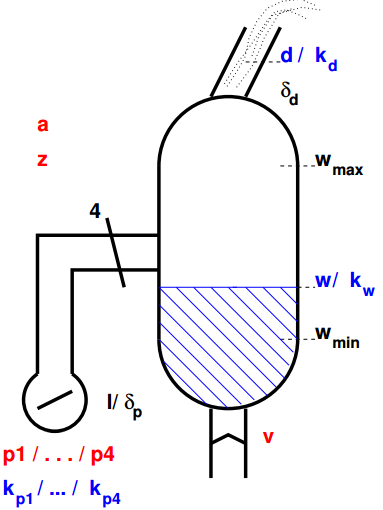
\includegraphics[scale=0.5]{Figures/Evaluation/steamboilerimage.png}
\caption{A diagram showing a theoretical Steamboiler. \label{fig:steamboiler}}
\end{figure}

An example of how the steamboiler could look is shown in figure
\ref{fig:steamboiler}. The variables of the steamboiler are shown in table
\ref{tab:steamboilervariables}.

\begin{table}[H]
\begin{tabular}{l|l}
\textbf{variables} & \textbf{description} \\
\hline
$w_{min}$ & minimal water level \\
$w_{max}$ & maximal water level \\
$l$ & water amount per pump\\
$d_{max}$ & maximal quantity of steam exiting the boiler \\
$\delta_{p}$ & error in the value of the pumps \\
$\delta_{d}$ & error in steam\\
$w$ & water level \\
$d$ &  amount of steam exiting the boiler \\
$k_{p,i}$ & pump $i$ works/broken \\
$k_{w}$ & water level measuring device works/broken \\
$k_{d}$ & steam amount measuring device works/broken\\
$p_{i}$ & pump $i$ on/off \\
$v$ & valve open/closed \\
$a$ & boiler on/off \\
$z$ & state init/norm/broken/stop 
\end{tabular}
\caption{The variables of the steamboiler and their descriptions. \label{tab:steamboilervariables}}
\end{table}

The full formal specification for the steamboiler is 10 pages long which can be
found in \cite{mathlangexamples}. Therefore we have given small examples taken
from the full specification.

\subsubsection{ZMathLang steps for the steamboiler case study.}

\begin{figure}[H]
\centering
\begin{minipage}{0.45\textwidth}
\centering
\includegraphics[scale=0.6]{{Figures/Evaluation}/0steamboilerimage.png}
\vspace{-0.18in}
\caption{The formal specification \LaTeX{} code for the steamboiler system. \label{fig:steamboiler0}}
\vspace{-0.2in}
\end{minipage}\hfill
\begin{minipage}{0.45\textwidth}
\centering
%[clip,l,b,r,t]
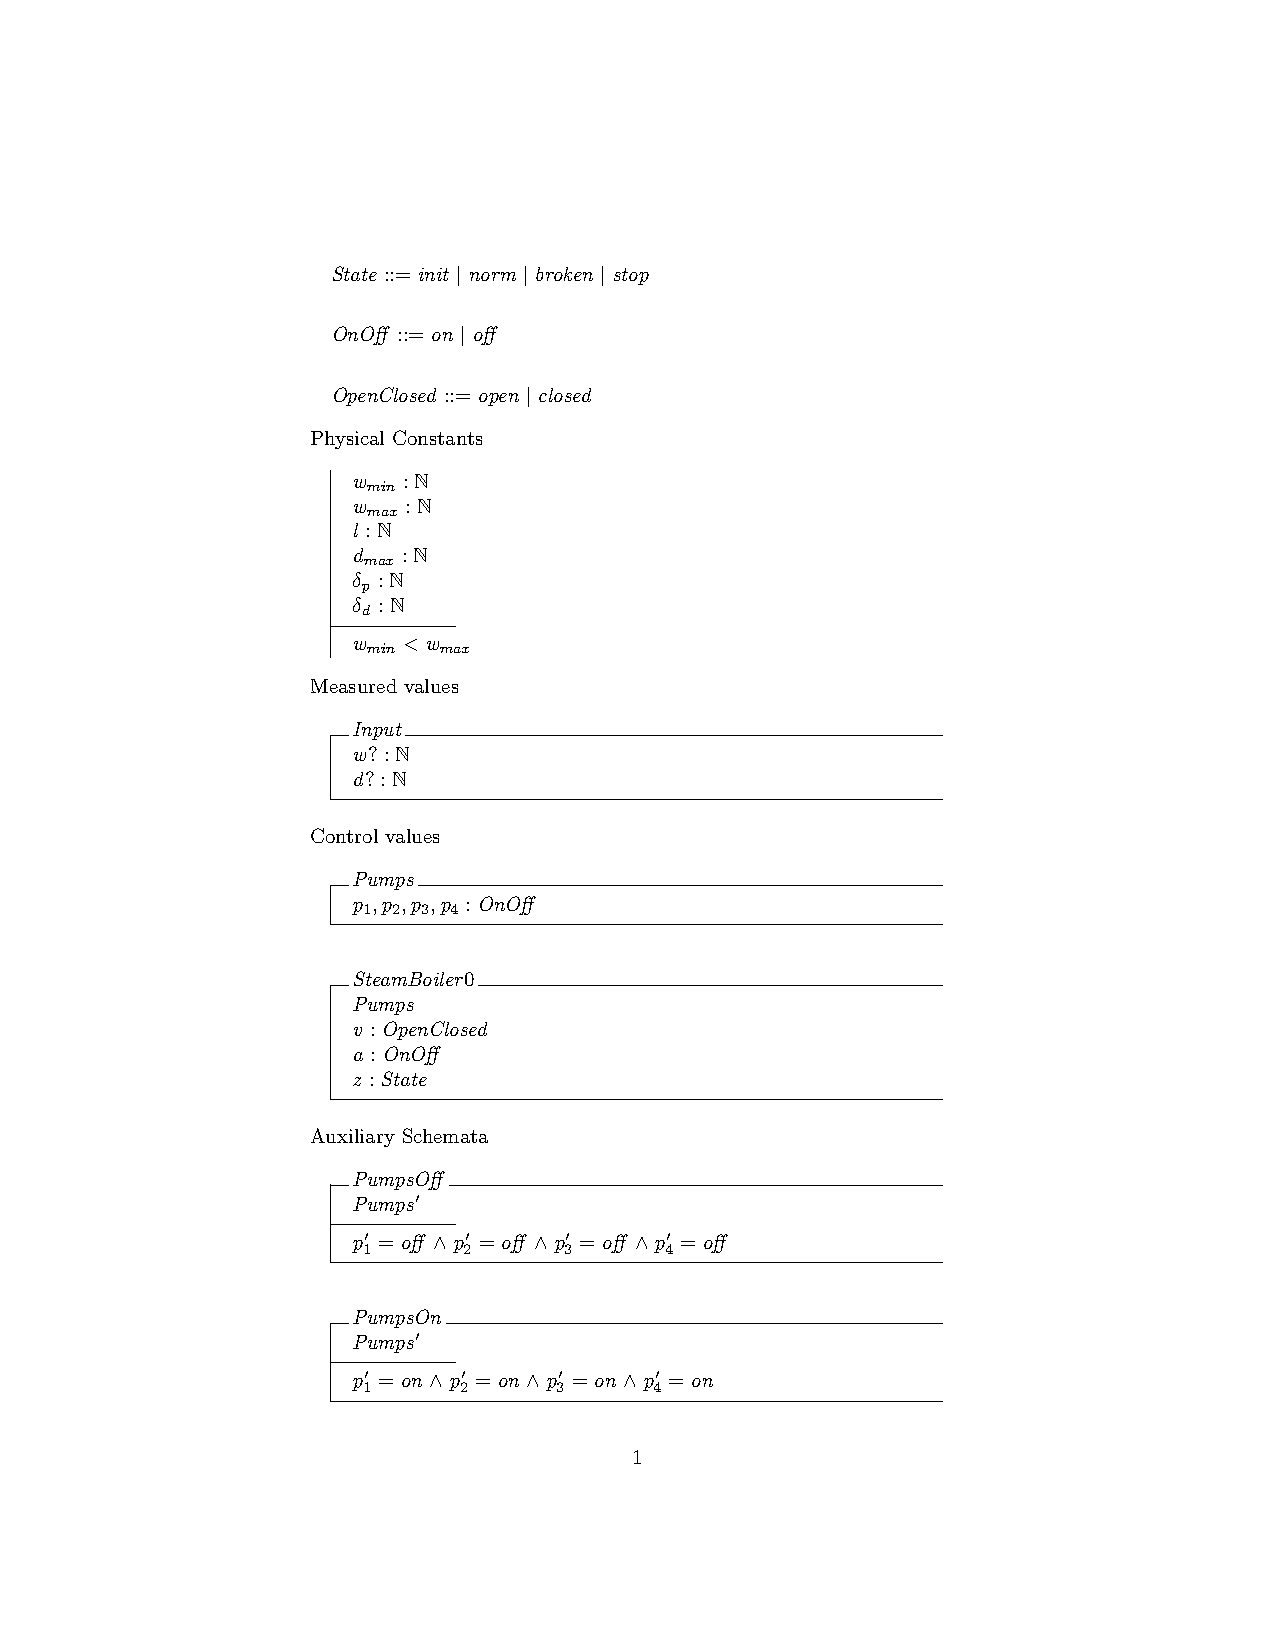
\includegraphics[clip, trim=5.5cm 4cm 5cm 4cm, scale=0.6]{examples/steamboiler/0.pdf}
\vspace{-0.2in}
\caption{The formal specification for the steamboiler system. \label{fig:steamboiler0comp}}
\vspace{-0.2in}
\end{minipage}
\end{figure}

We show the \LaTeX{} code for part of the raw steamboiler specification in
figure \ref{fig:steamboiler0} and it's pdflatex counterpart in figure
\ref{fig:steamboiler0comp}.

We then annotate the specification using \gls{zcga} and \gls{zdra} labels.

\begin{figure}[H]
\centering
\begin{minipage}{0.45\textwidth}
\centering
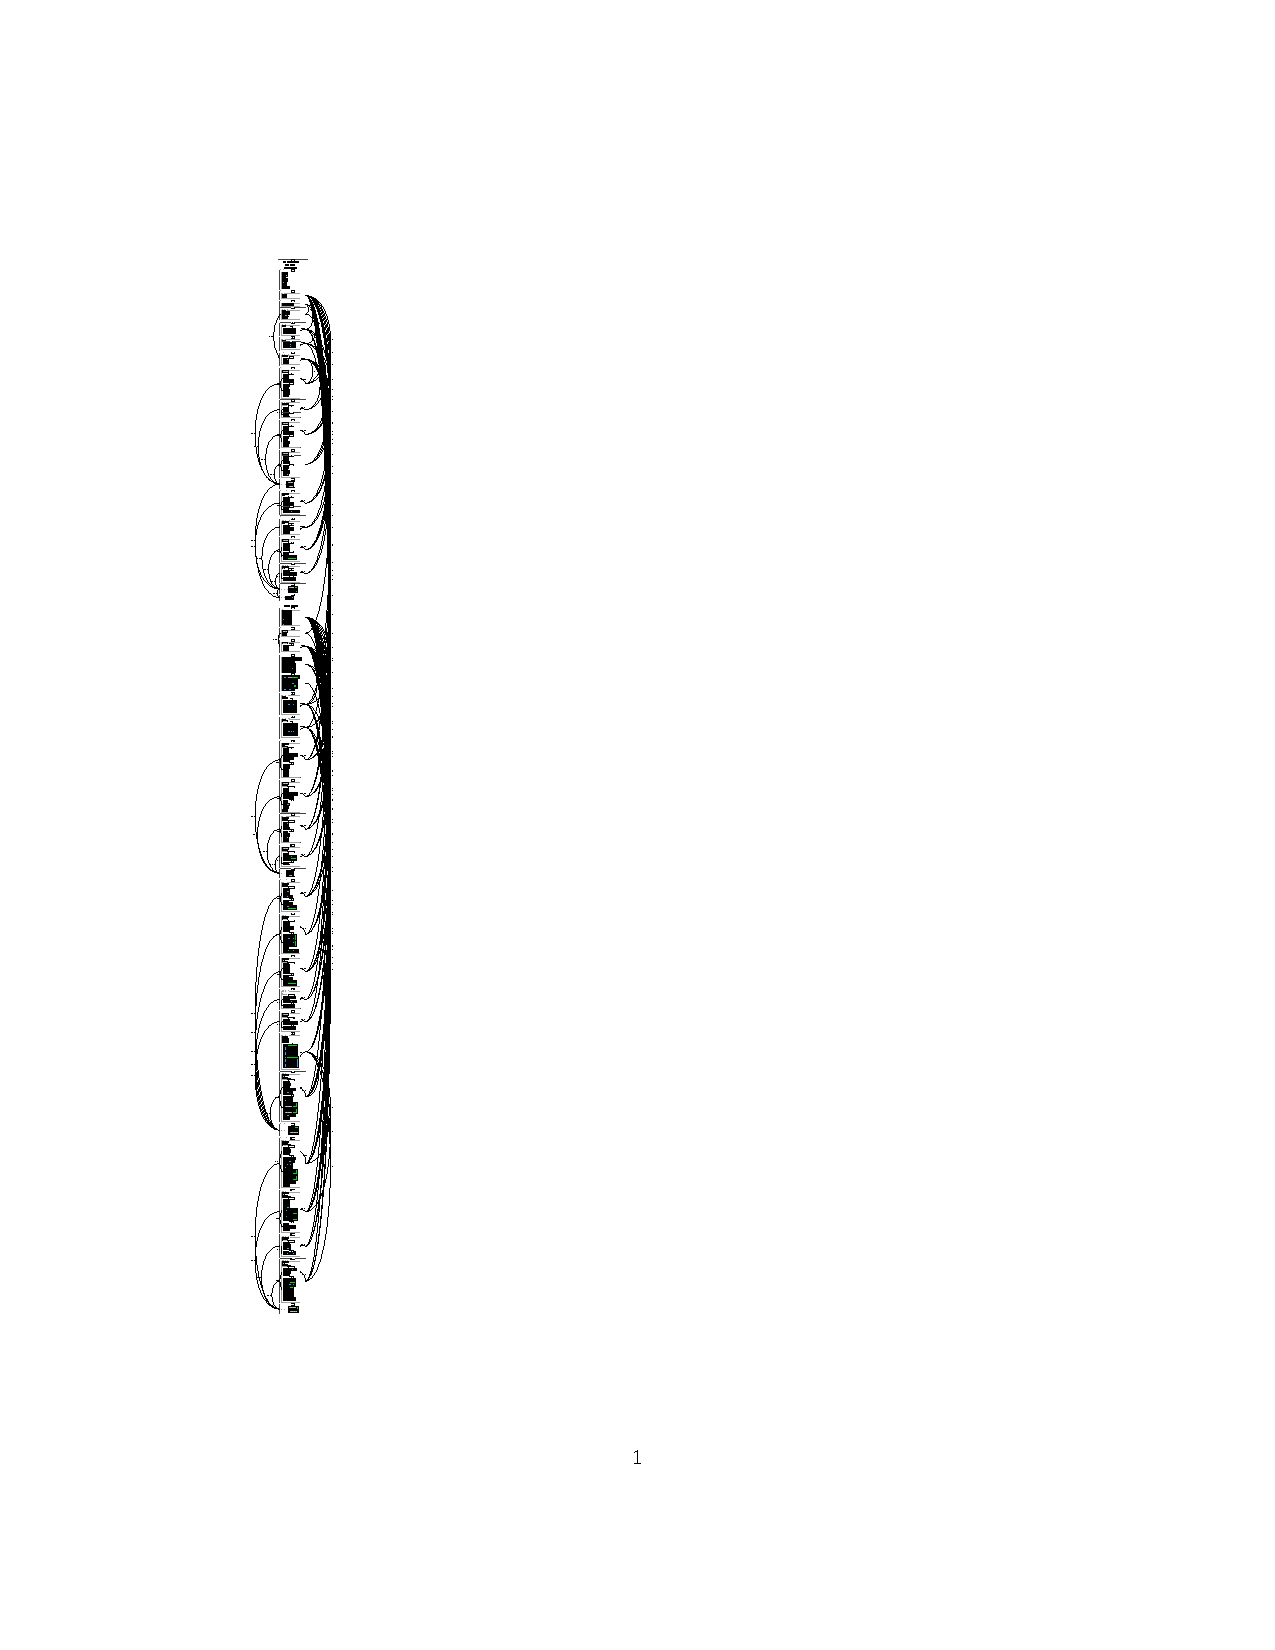
\includegraphics[clip, trim=3cm 8cm 6cm 2cm]{examples/steamboiler/1n2.pdf}
\vspace{-0.18in}
\caption{An example of the original steamboiler specification annotated in \gls{zcga} and \gls{zdra}. \label{fig:steamboilert1n2}}
\vspace{-0.2in}
\end{minipage}\hfill
\begin{minipage}{0.45\textwidth}
\centering
%[clip,l,b,r,t]
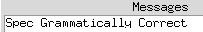
\includegraphics[width=7cm]{examples/steamboiler/zcgacorrect.png}

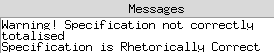
\includegraphics[width=7cm]{examples/steamboiler/zdracorrect.png}

\caption{The result when checking the steamboiler specification with the \gls{zcga} and \gls{zdra} checkers. \label{fig:steamboilercorrect}}

\end{minipage}
\end{figure}

Since we only have a warning and no errors when checking the steamboiler
specification we can now generate a goto graph and dependency graphs for it.

\begin{figure}[H]
\centering
\begin{minipage}{0.45\textwidth}
\centering
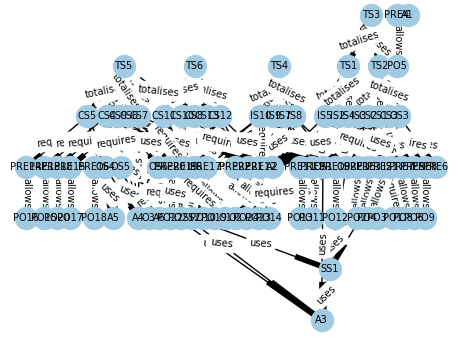
\includegraphics[trim=4cm 1cm 1cm 1cm, scale=0.5]{Figures/Evaluation/25a.png}
\caption{The dependency graph produced for the steamboiler specification. \label{fig:steamdepgraph}}
\end{minipage}\hfill
\begin{minipage}{0.43\textwidth}
%[clip,l,b,r,t]
\centering
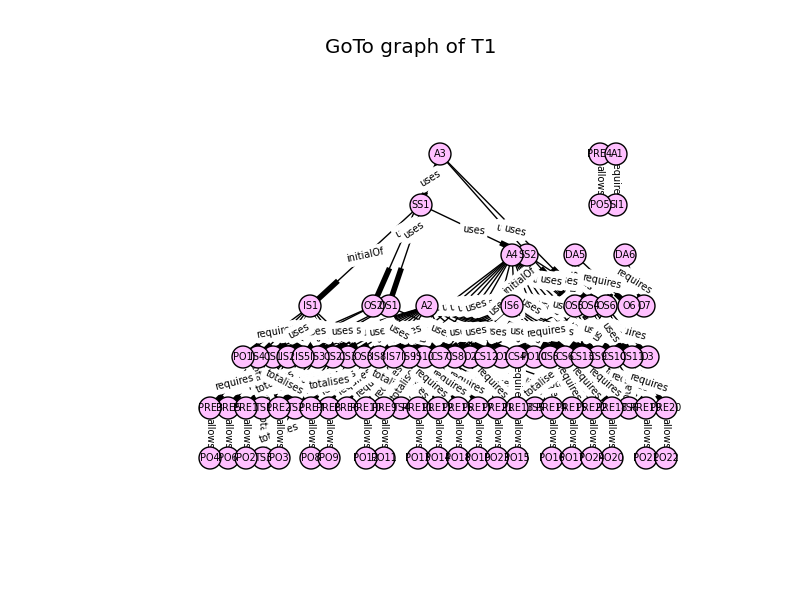
\includegraphics[trim=4cm 1cm 1cm 1cm, scale=0.5]{examples/steamboiler/25b.png}
\caption{The goto graph produced for the steamboiler specification. \label{fig:steamgotograph}}
\end{minipage}
\end{figure}

The dependency and goto graphs are shown in figures \ref{fig:steamdepgraph} and
\ref{fig:steamgotograph} respectively. Since there are a lot of \gls{zdra}
instances and therefore a lot of nodes, both the dependency graph and goto graph
are cluttered. One way to solve this is to use zooming facilities for graphs.
However, as the program at the moment outputs the graphs as `.png' files, the
program will need to be modified in a way so that the graphs are produced in a 
different file format for graph exploration.
 We will discuss this as a limitation in the next section.

From the goto graph the \gls{zmath} tool kit automatically generates a general
proof skeleton, which uses the order from the goto graph to order the instances
in how they should appear in any theorem prover. Part of the skeleton for the
steamboiler specification is shown in figure \ref{fig:steamgpsa}.

\begin{figure}[H]
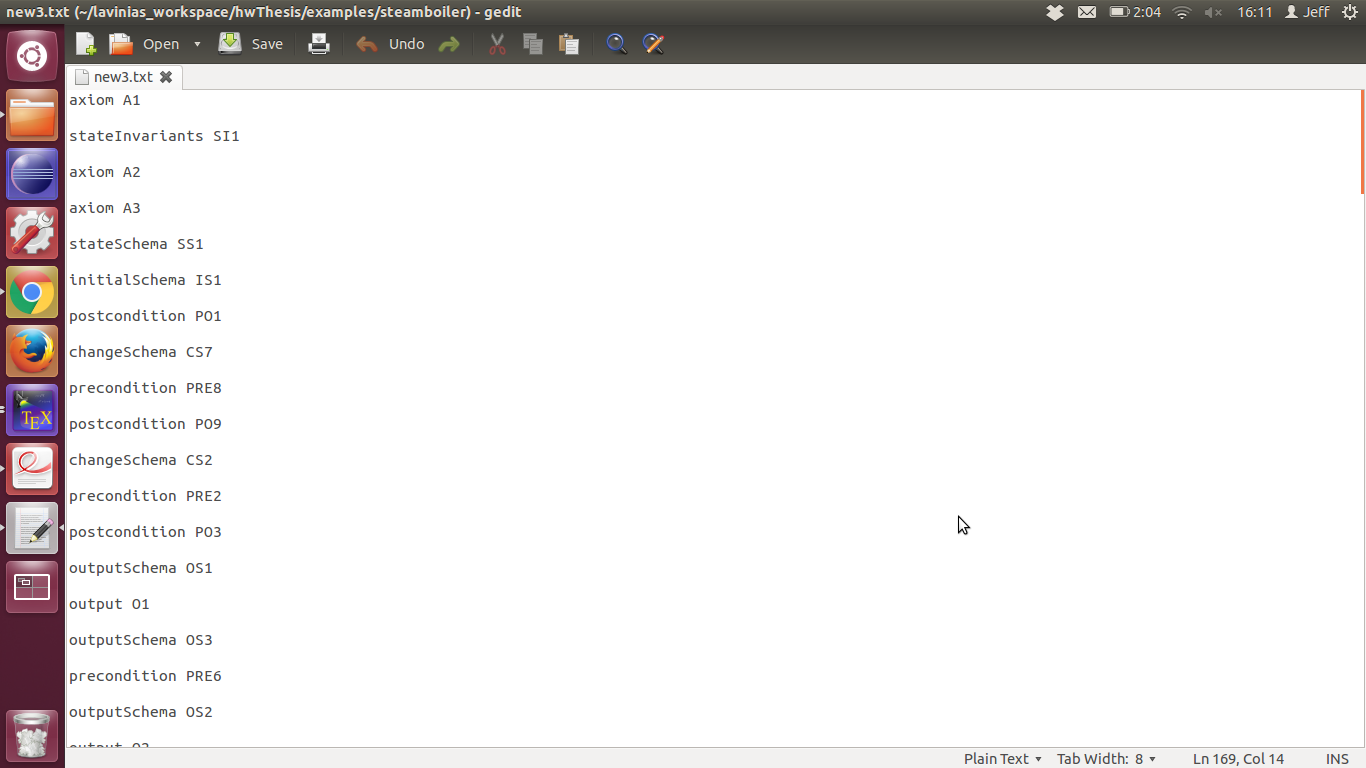
\includegraphics[scale=0.5]{Figures/Evaluation/steamboilergpsa.png}
\caption{\Gls{gps} for the steamboiler specification. \label{fig:steamgpsa}}
\end{figure}

We can now translate the \gls{gps} into Isabelle syntax using the \gls{zmath}
tool-kit.

\begin{figure}[H]
    \hfill
    \subfigure{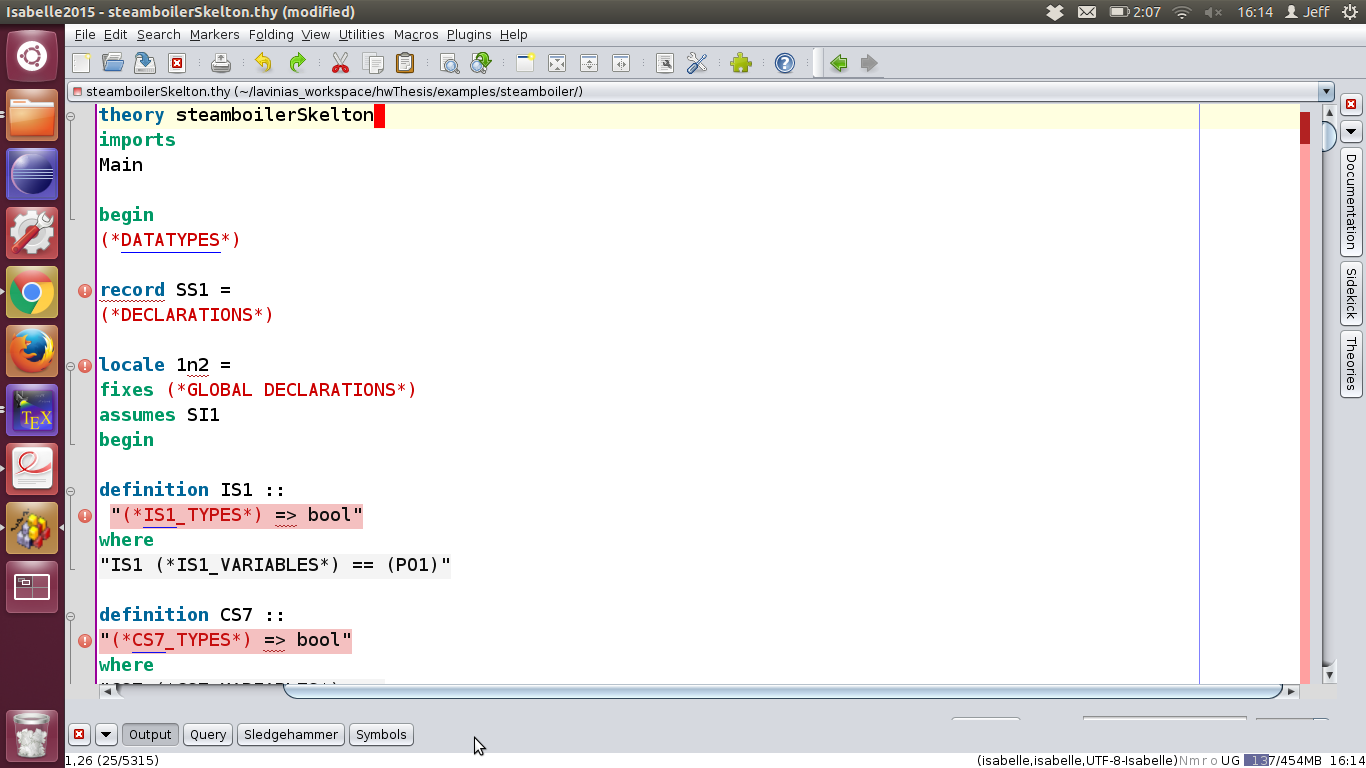
\includegraphics[width=6cm]{Figures/Evaluation/4image.png}}
    \hfill
    \subfigure{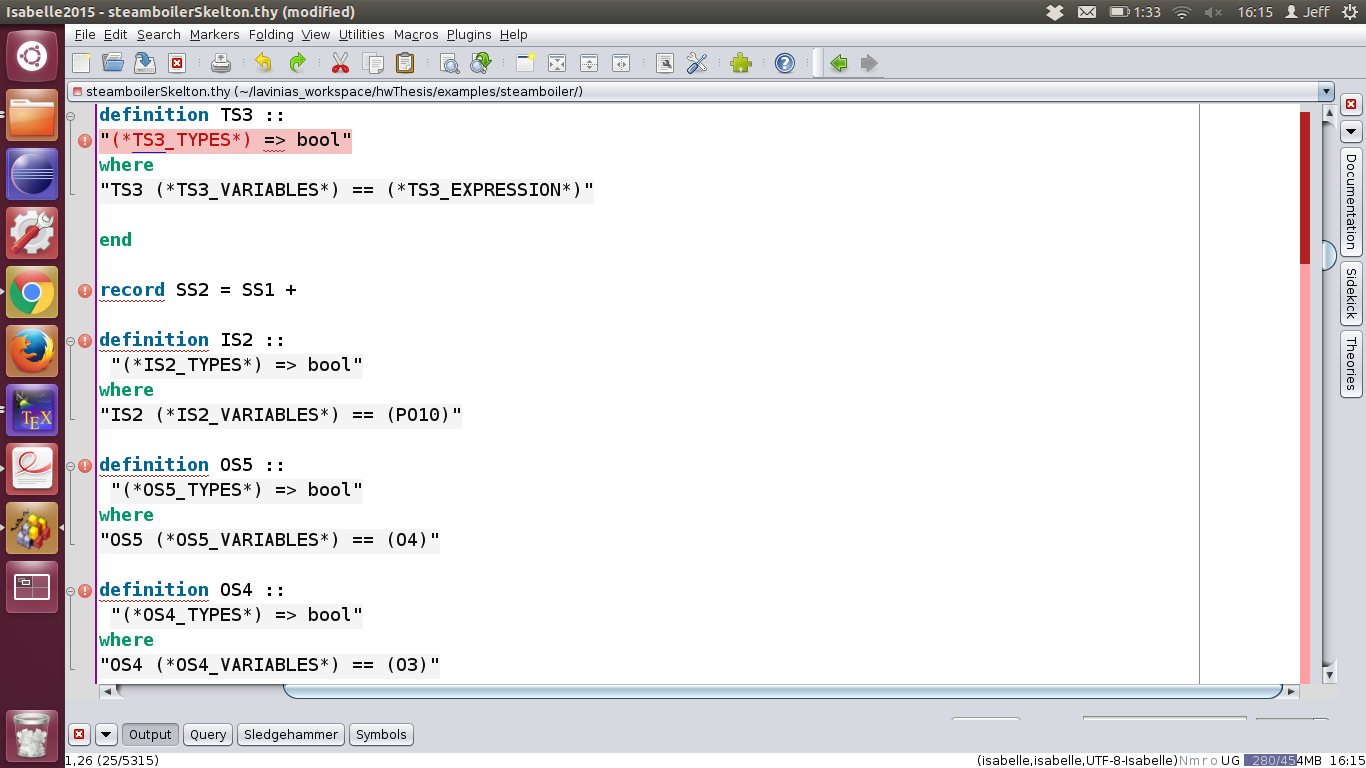
\includegraphics[width=8cm]{Figures/Evaluation/4imageb.png}}
    \hfill
    \caption{Part of the isabelle skeleton for the steamboiler specification.\label{fig:steamisaskel}}
\end{figure}

Part of the isabelle skeleton for the steamboiler specification is shown in
figure \ref{fig:steamisaskel}. Since the steamboiler example has 2 stateSchema's
the \gls{zmath} tool-set creates 2 isabelle 	\texttt{records} in the theory file.
The top left image shows the beginning part of the isabelle skeleton, where the
first stateSchema (or record) sets the state of the theory. Midway down the
theory file the first record \texttt{ends} and a new one is added with the line
\verb|record SS2 = SS1 +|. Towards the end the isabelle skeleton there are
lemma's to check the consistency for all state changing schema's (\texttt{CS})
in the format described in chapter \ref{ch:skeletons} section \ref{subsec:pob1}.
Using the \gls{zcga} annotated specification and the steamboiler isabelle
skeleton, the \gls{zmath} tool support can now fill in the isabelle skeleton the
declarations, expressions, schemaNames etc.

\begin{figure}[H]
    \hfill
    \subfigure{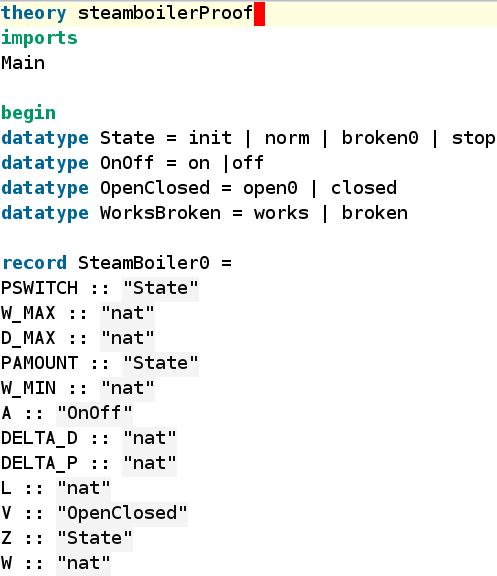
\includegraphics[width=7cm]{Figures/Evaluation/5imagea.png}}
    \hfill
    \subfigure{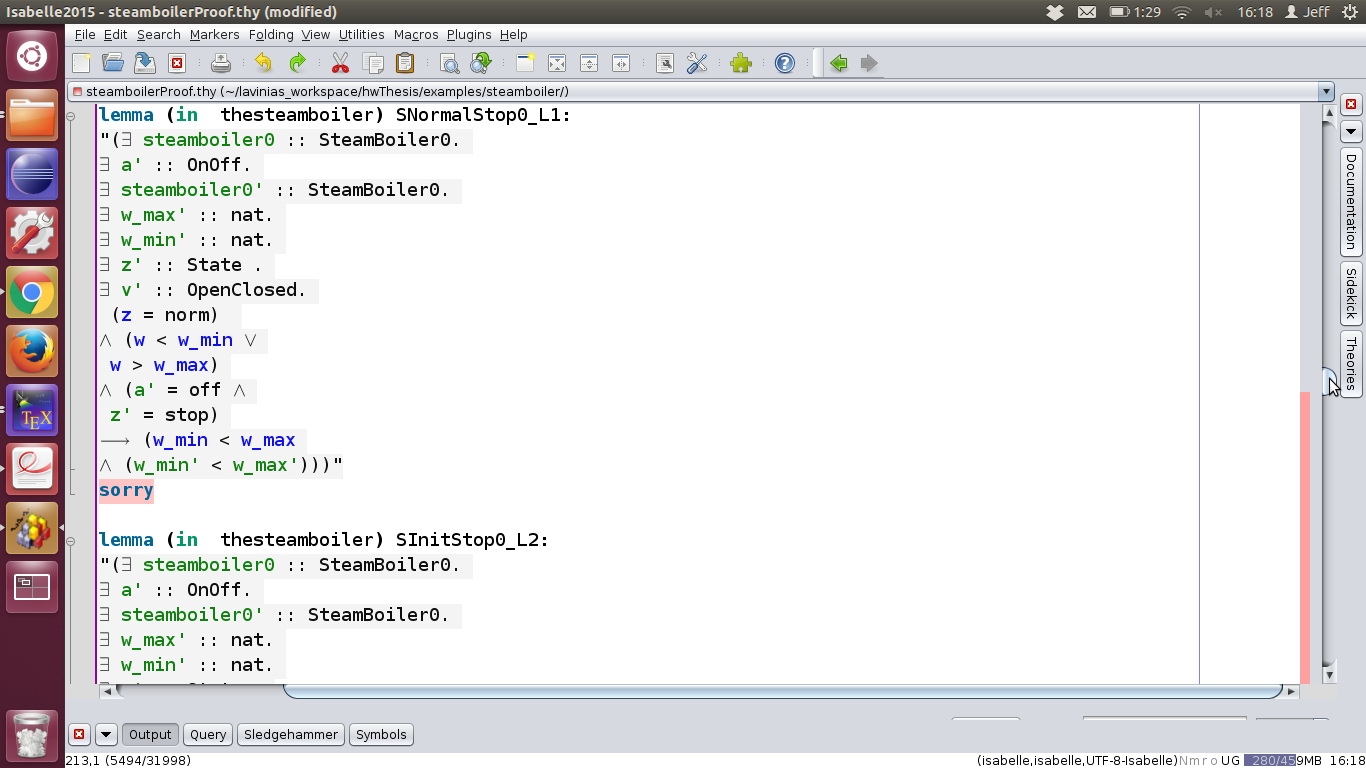
\includegraphics[width=7cm]{Figures/Evaluation/5imagec.png}}
    \hfill
    \caption{Part of the filled in isabelle skeleton for the steamboiler specification.\label{fig:filledinsteamskeleton}}
\end{figure}

In figure \ref{fig:filledinsteamskeleton} we show 3 parts of the filled in
isabelle skeleton (\gls{half}). The first part shows the beginning of the
\gls{half} which initiates the beginning of the proof. Since $SS1$ in this case
was the root of the tree in the goto graph it sets \verb|SteamBoiler0| as the
first record. Half way through the theory file we see another record,
\verb|SteamBoiler1| which was $SS2$ in \gls{zdra}. This is shown in the bottom
picture in figure \ref{fig:filledinsteamskeleton}. $SS2$ introduced 2 new state
variables, $S$ and $delta$ which are added to the new record. Towards the end of
the \gls{half}, \gls{zmath} has filled in the lemma's to prove which are sanity
checks for the specification.
The sanity checks for the steamboiler specification check that all 21 of the 
steamboiler `\textit{changeSchema's}' do not conflict with the stateInvariants.
So after every change in state $w_{min}<w_{max}$.
It fills in the lemma's with the correct syntax so
that the user only needs to delete the word `\emph{sorry}' prove the properties
in order to get a proof of their specification. 

\begin{figure}[H]
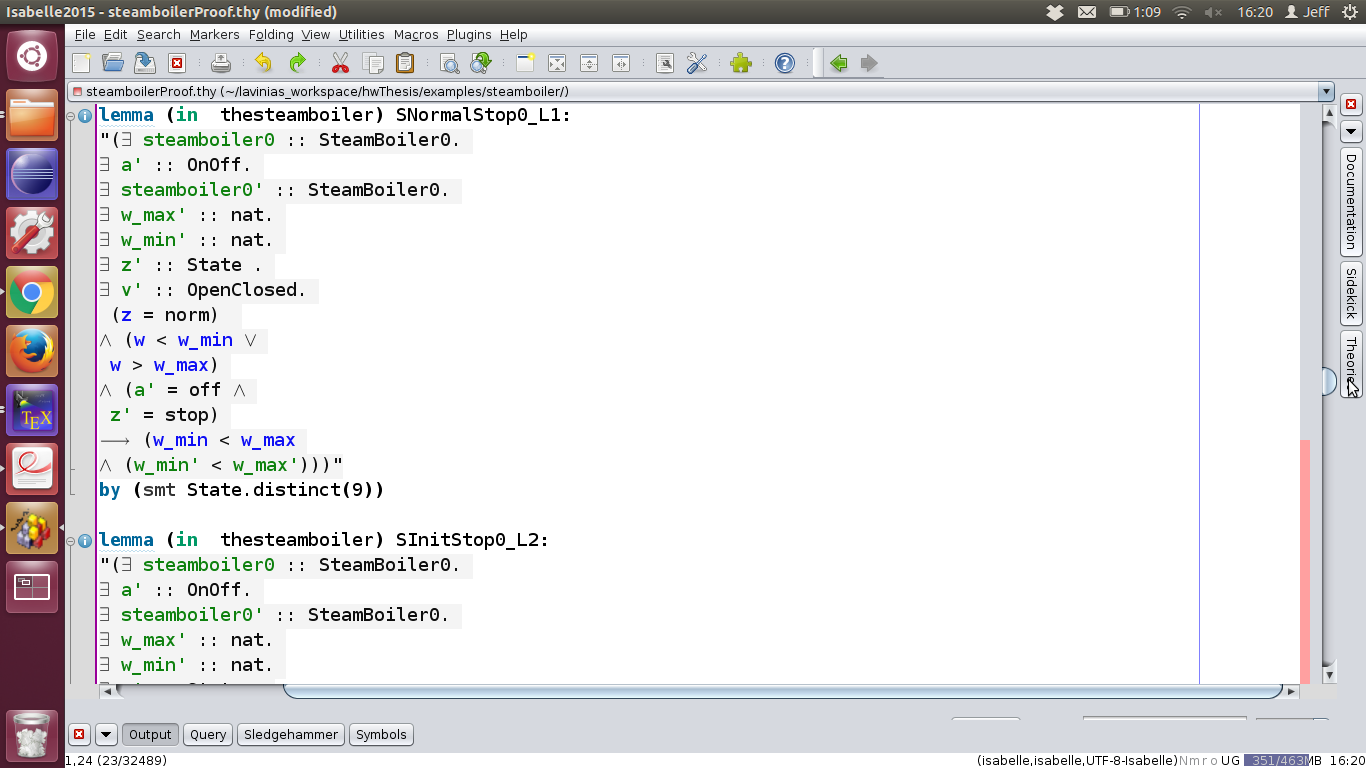
\includegraphics[scale=0.5]{Figures/Evaluation/6image.png}
\caption{Manually proven lemma for the steamboiler specification. \label{fig:steamboilerproof}}
\end{figure}

Using the lemma's which have been generated in figure
\ref{fig:filledinsteamskeleton} we have proved all of these lemmas for the
steamboiler specification, part of which is shown in figure
\ref{fig:steamboilerproof}. By doing so, we have now proven that non of the
state changing schemas conflict with the state invariants of the specification.
To do this we have manually deleted the `\emph{sorry}' command, used the Isar
tool `\emph{sledgehammer}' which has indicated that to prove this particular
lemma (shown in figure \ref{fig:steamboilerproof}) it can be proven by
\verb|smt State.distinct(9)|.
Therefore it is true that the `\texttt{SNormalStop0}' schema
does not conflict with the state Invariants. We did this step manually for all
remaining lemmas, the full proof of the steamboiler specification can be found
in \cite{mathlangexamples}.


In \cite{laibinis} a link between safety requirements, event-B models and corresponding fragments of
a safety case is created. Laibinis et al present a method and tool support linking formal modelling in
Event-B and safety case construction. Whereas \gls{zmath} translates formal modelling into the Isabelle 
theorem prover which can then be used as evidence to create a safety case for high integrity systems.
Laibinis paper employs refinement to create proofs (point 5 from figure \ref{fig:ptp}) whereas \gls{zmath}
employs sanity and consistency checks (points 1 and 2 from figure \ref{fig:ptp}). Refinement proofs requires
refinement specifications to be present in order to develop the proofs. The aim of \gls{zmath} was to be able
to create proofs for specifications which are also semi-formal and therefore creates proofs sanity and consistency
instead.

In \cite{laibinis} SteamBoiler example, Laibinis et al uses an abstract specification as well as 
4 other refinement specifications. \Gls{zmath} can translate an abstract specification and creates 
proof obligations without a refinement specification. Safety requirements are added and translated 
into event-B. An example of such a safety requirement is `\textit{during system operation the water level shall not exceed the
predefined safety boundaries}'. In \gls{zmath} additional safety requirements to prove can also be added
and written in Isabelle.

One advantage of using \cite{laibinis} to prove the SteamBoiler specification is that the SteamBoiler
has been written in Event-B which is supported by the Rodin platform to prove refinements and
 that this technique has been used by industry.
 However a disadvantage of using this technique is that in order to create proofs one must have refinement
 specifications as well as an abstract specification. The specification must also be a completed finished product.
 An advantage of the \gls{zmath} toolkit is that one can do proofs on a single abstract specification, and the 
 proofs can also be done on specification which aren't complete and ones which are semi-formalised.
 Another advantage of using \gls{zmath} is that the steamboiler can undergo other checks (ZGa, ZDRa) just
 using the abstract specification. So the specification doesn't need refinement specifications. The diagrams
 and results produced (dependency graphs, GoTo graphs etc) can also be presented as evidence within the safety case.
 However, to get this evidence the user will need to label the specification which could be argued as a little tedious.
 A disadvantage of using \gls{zmath} to prove the Steamboiler specification is to generate a solid safety case
 one needs to add safety related requirements in Isabelle.

\subsection{Case Study 2: A specification using both terms and sets.}

This case study based is on the \emph{ModuleReg} specification which uses both
terms and sets. The specification has been translated into Isabelle using the
\gls{zmath} framework. The entire \gls{zmath} works for the ModuleReg example is
shown in chapter \ref{ch:fullexample}.

The \emph{ModuleReg} specification is our smallest example with 43 lines of
\LaTeX{} code, 1 \emph{zed} environment and 3 \emph{schema}'s. There are 20
labels of \emph{schemaText}, 6 \emph{declarations}, 18 \emph{expressions}, 13
\emph{terms}, and 31 \emph{sets}. Since there are \emph{stateInvariants} for the
\emph{modulereg} specification, \gls{zmath} was able to generate lemma's to
prove for the 2 \emph{changeSchemas}. There is also 1 \emph{stateSchema}, 2
\emph{preconditions} and 2 \emph{postconditions}. There are 3 \emph{requires}
relations, 2 \emph{allows} and 2 \emph{uses}.

Since the \emph{modulereg} specification is quite small but did have
stateInvariants which \gls{zmath} could prove are satisfied throughout the
specification, we decided it would be a could example to show the full workings
of. This is shown in chapter \ref{ch:fullexample}.

In conclusion there is not much difference in the difficulty of translation
between those specifications using just terms and those specifications using
both terms and sets.

\subsection{Case Study 3: A semi formal specification.}

In this case study we present the \emph{AutoPilot} specification. The
specification is a semi formal specification and has been partially translated
into Isabelle. The parts which have been translated are written formally and
have been annotated accordingly. This gives an example of a specification which
is written in natural language and is on it's way to being formalised.

We have taken the natural language specification for an autopilot system from
\cite{Butler96} and started to formalise it.

\begin{figure}[H]
\centering
\begin{minipage}{0.45\textwidth}
\centering
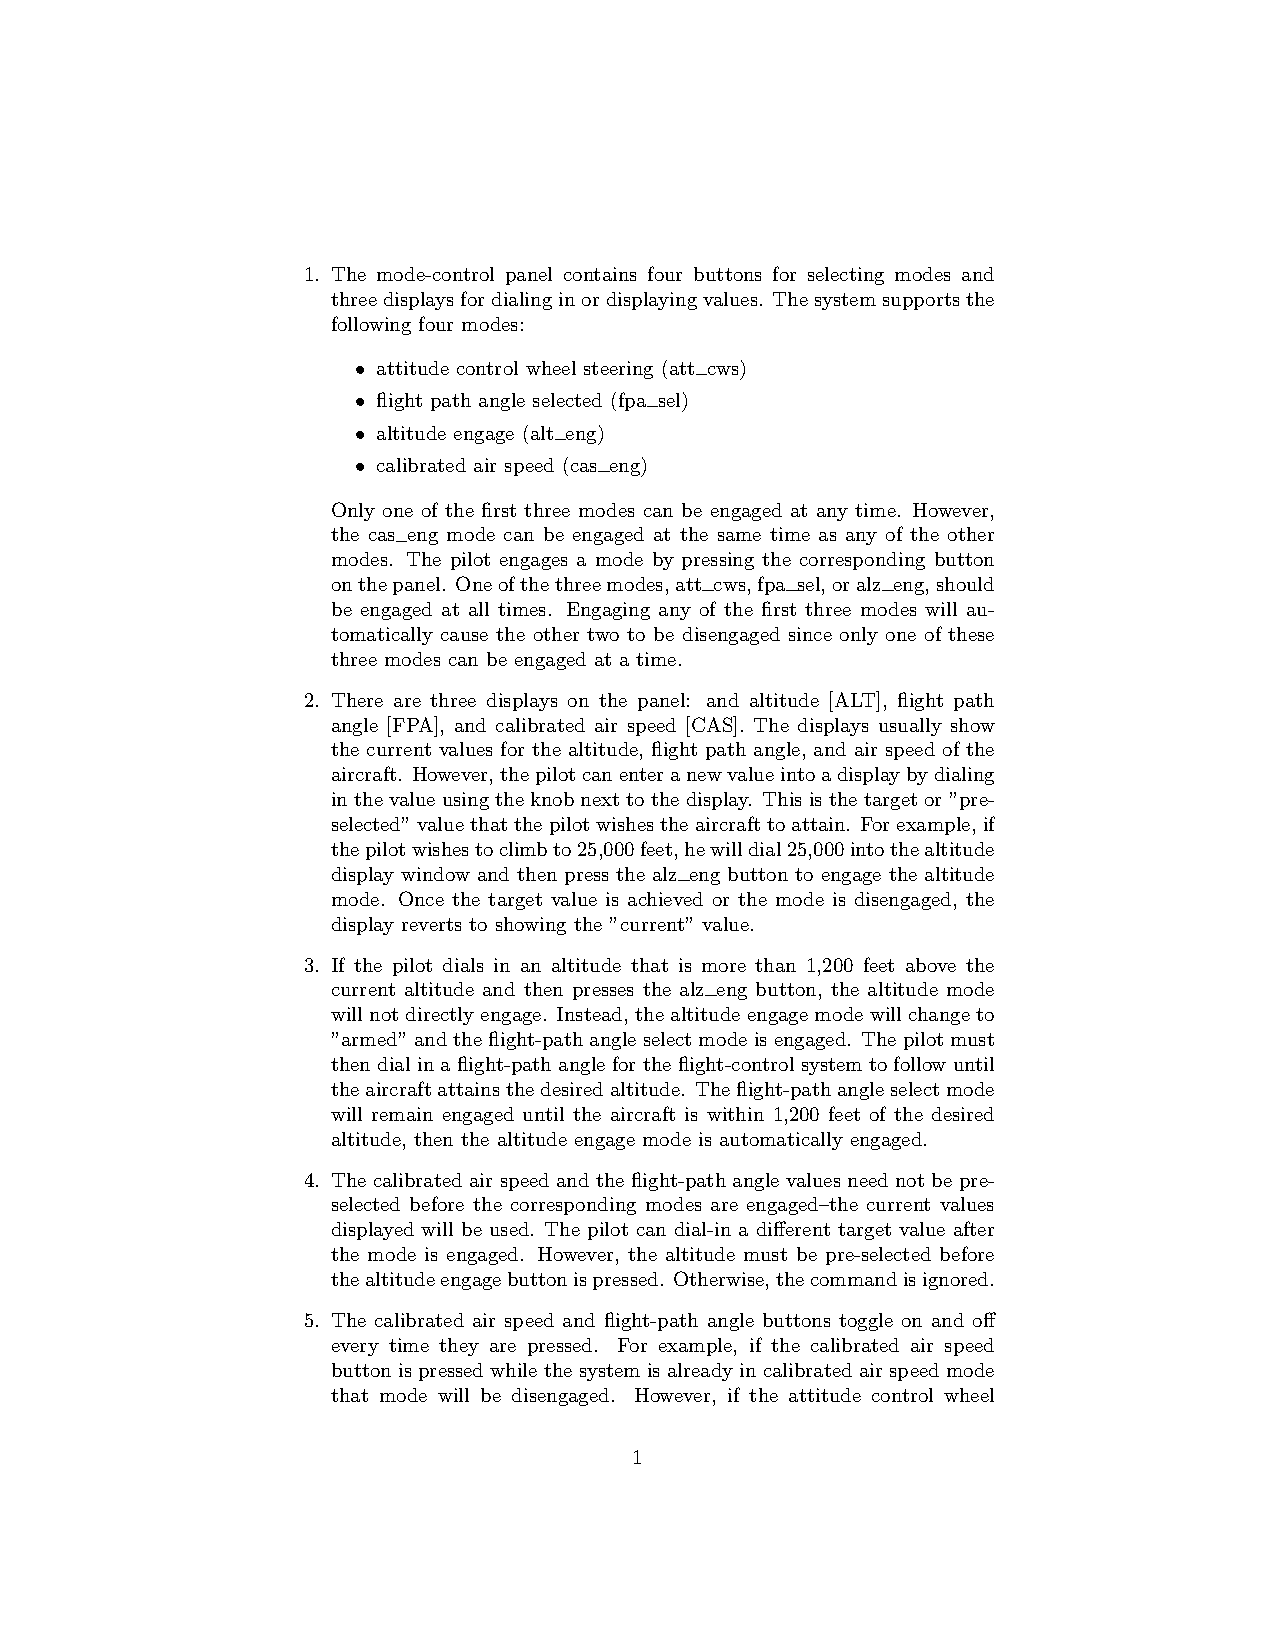
\includegraphics[clip, trim=5.5cm 11cm 4cm 4.5cm, scale=0.6]{examples/semiform/informal.pdf}
\vspace{-0.18in}
\caption{An example of the original Autopilot specification. \label{fig:originalautopilot}}
\vspace{-0.2in}
\end{minipage}\hfill
\begin{minipage}{0.45\textwidth}
\centering
%[clip,l,b,r,t]
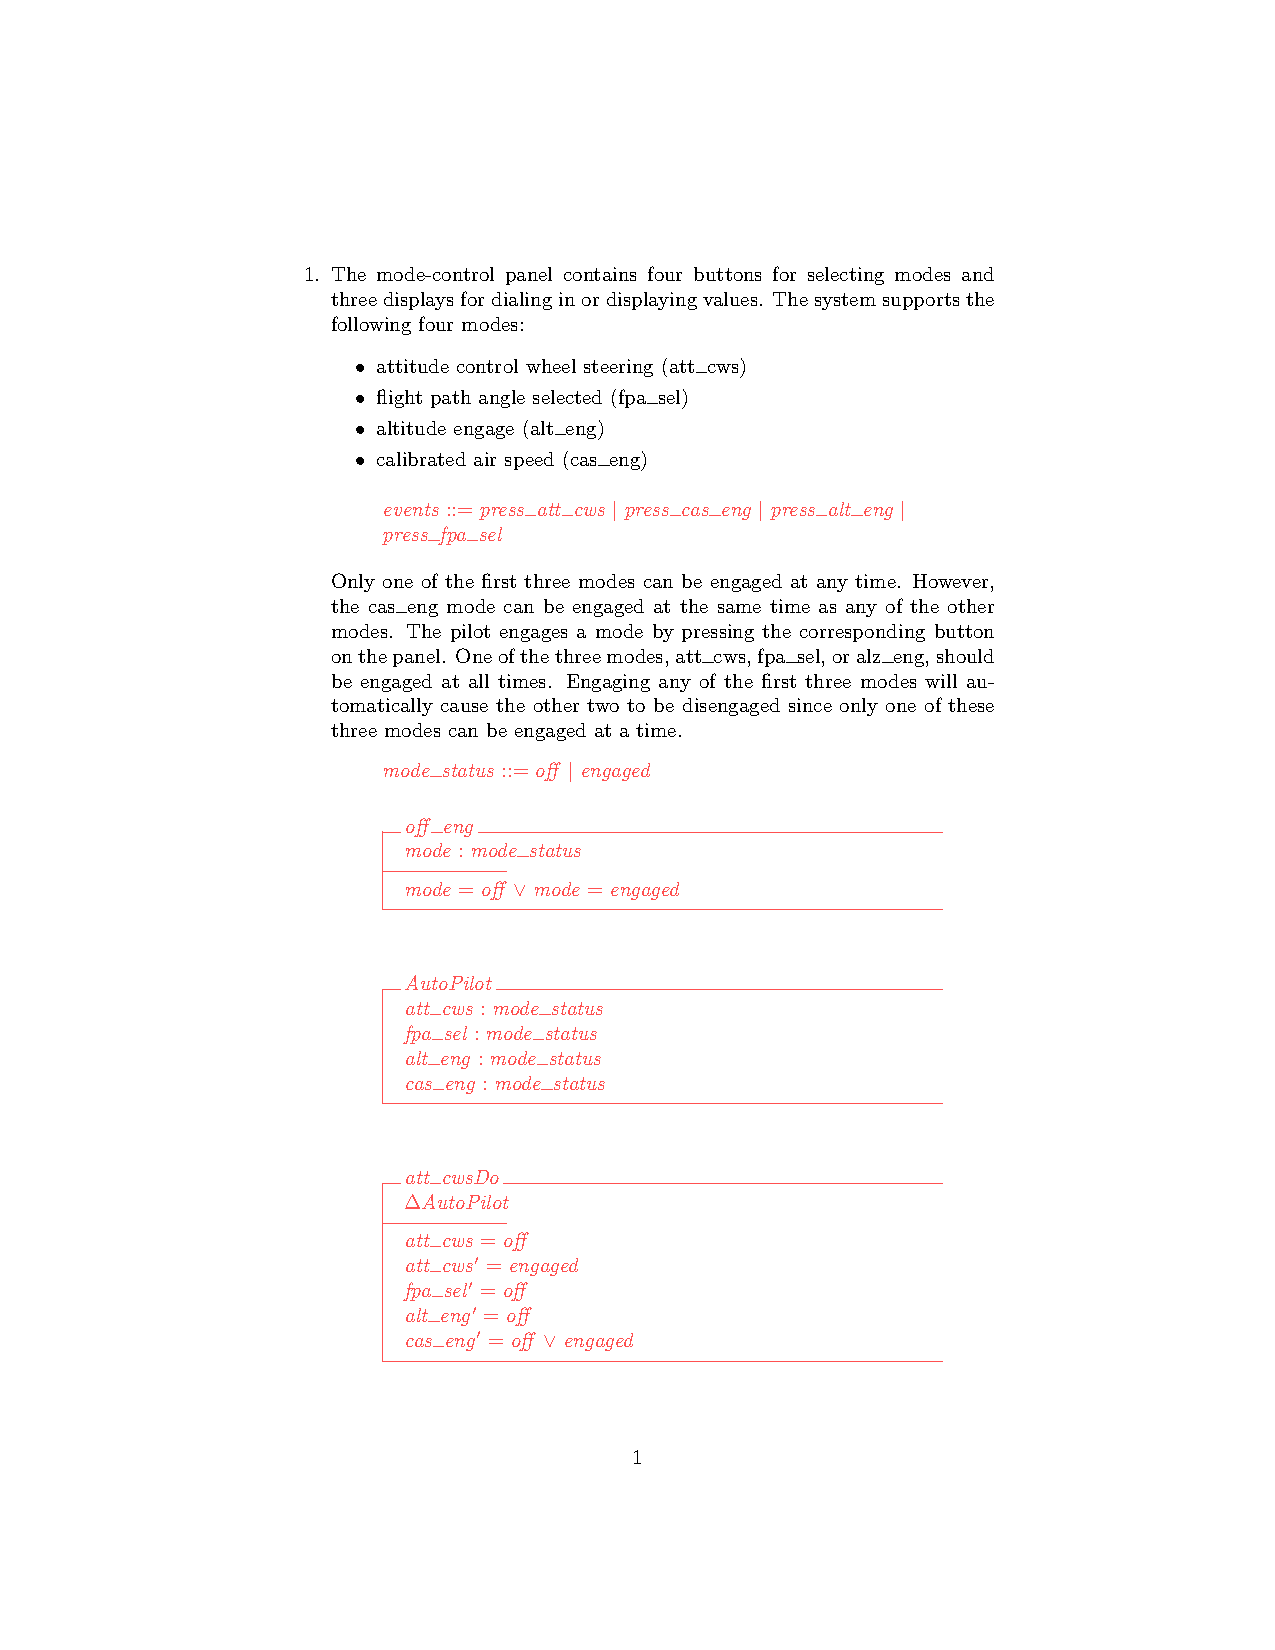
\includegraphics[clip, trim=5.5cm 11cm 4cm 4.5cm, scale=0.6]{examples/semiform/semiformal.pdf}
\vspace{-0.2in}
\caption{An example of the Autopilot specification partially formalised. \label{fig:semiformautopilot}}
\vspace{-0.2in}
\end{minipage}
\end{figure}


\subsubsection{ZMathLang steps for the autopilot case study.}

We give the informal specification in figure \ref{fig:originalautopilot} and one
which we are beginning to formalised in figure \ref{fig:semiformautopilot}. We
have highlighted in {\color{set}red} the parts which we have formalised in
figure \ref{fig:semiformautopilot}. The formalised parts of the semi formal
specification are taken from the text in the informal specification.

We then annotate the partial formal specification in \gls{zcga} annotations and
\gls{zdra} annotations taken from chapters \ref{ch:zcga} and \ref{ch:zdra}
respectively. Once annotated we can check the annotated document for \gls{zcga}
and \gls{zdra} errors. 

\begin{figure}[H]
\centering
\begin{minipage}{0.45\textwidth}
\centering
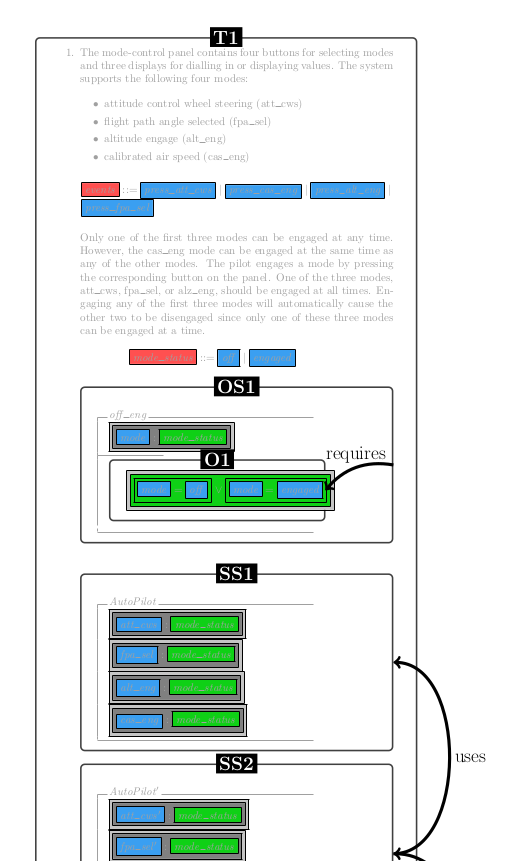
\includegraphics[width=7cm]{examples/semiform/1n2.png}
\vspace{-0.18in}
\caption{An example of the original Autopilot specification annotated in \gls{zcga} and \gls{zdra}. \label{fig:autopilot1n2}}
\vspace{-0.2in}
\end{minipage}\hfill
\begin{minipage}{0.45\textwidth}
\centering
%[clip,l,b,r,t]
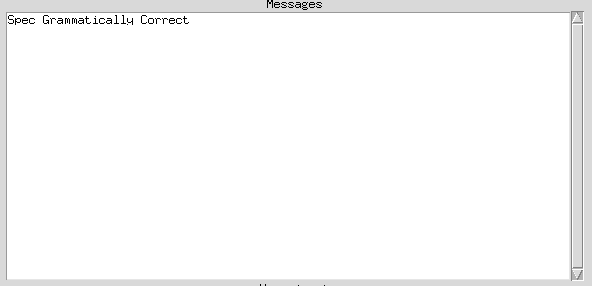
\includegraphics[width=7cm]{examples/semiform/zcgacorrect.png}
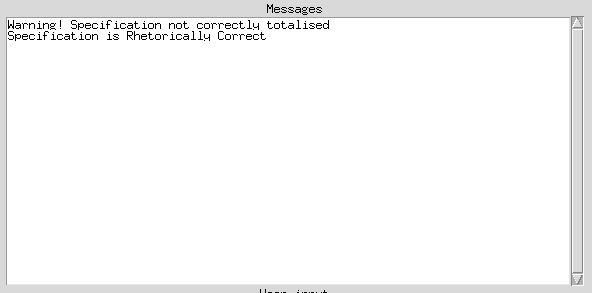
\includegraphics[width=7cm]{examples/semiform/zdracorrect.png}
\vspace{-0.2in}
\caption{The result when checking the autopilot specification with the \gls{zcga} and \gls{zdra} checkers. \label{fig:autopilotcorrect}}
\vspace{-0.2in}
\end{minipage}
\end{figure}

Even though the specification is not fully formalised we can still annotate it
with \gls{zcga} and \gls{zdra} and check for the correctness of the parts which
have been annotated (shown in figures \ref{fig:autopilot1n2} and
\ref{fig:autopilotcorrect}). When checking with \gls{zdra} we have a warning
message telling the user that the specification is not correctly totalised.
We remind the reader that a specification is `\textit{not correctly totalised}' when 
every preconditions has a corresponding postcondition or output (section \ref{subsec:correctlytotalised}). 
This does not matter for now in our semi-formal specification
as we can still carry on with the translation.

When checking the specification for \gls{zdra}, \gls{zmath} has also produced a
dependency graph and goto graphs (shown in figures \ref{fig:autodepgraph} and
\ref{fig:autogotograph}):

\begin{figure}[H]
\centering
\begin{minipage}{0.45\textwidth}
\centering
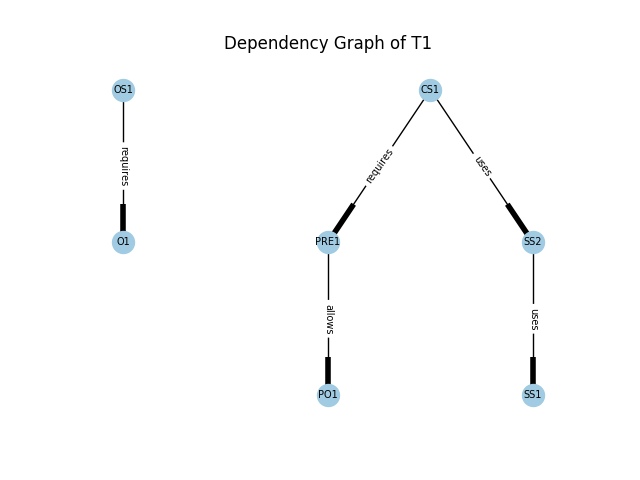
\includegraphics[scale=0.5]{Figures/Evaluation/semiform25a.png}
\vspace{-0.18in}
\caption{The dependency graph produced for the autopilot specification. \label{fig:autodepgraph}}
\vspace{-0.2in}
\end{minipage}\hfill
\begin{minipage}{0.43\textwidth}
\centering
%[clip,l,b,r,t]
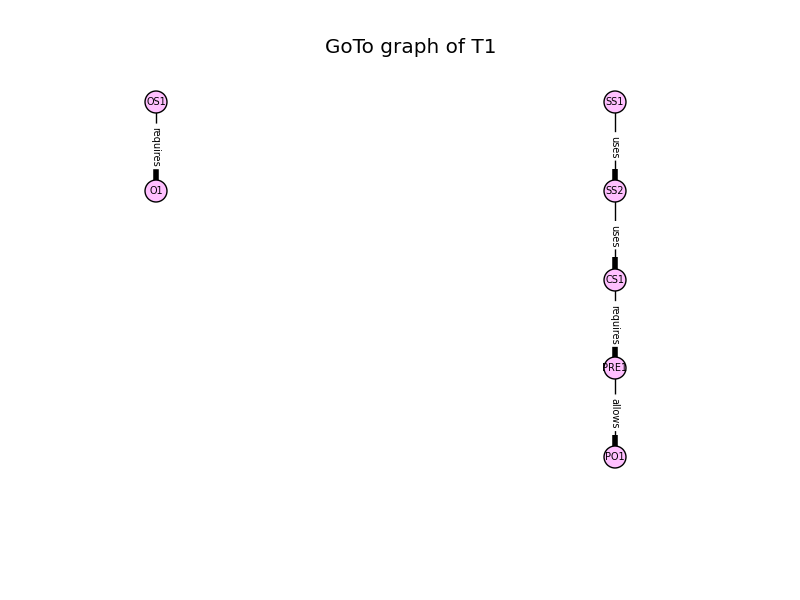
\includegraphics[scale=0.5]{examples/semiform/25b.png}
\vspace{-0.2in}
\caption{The goto graph produced for the autopilot specification. \label{fig:autogotograph}}
\vspace{-0.2in}
\end{minipage}
\end{figure}

With the dependency graph (figure \ref{fig:autodepgraph}) we can say that $SS2$
uses $SS1$, $CS1$ uses $SS2$, $PRE1$ requires $CS1$ and allows $PO1$. Which
makes up the main tree dependencies. $OS1$ and $O1$ are separate as they do not
have any relations which any parts of the main tree, the only dependency they
have is on each other where $O1$ requires $OS1$.

We can say that the dependency graph \emph{describes} the relation between
instances and the goto graph (figure \ref{fig:autogotograph}) \emph{orders} the
instances in a way as to parse through a theorem prover.

We can now generate a general proof skeleton for the Autopilot specification
even though it is not fully formalised (shown in figure \ref{fig:autopilotgps}).
We can clearly see that the arrow has changed direction for the $OS1$ and $O1$
relationship from the dependency graph. Again since these two instances are not
dependency on any part of the main tree they are separate. However in the
dependency graph described the relation that $O1\ requires\ OS1$ ($O1$ root and
$OS1$ child) the goto graph flips this relationship as in a theorem prover we
would need $OS1$ to appear before $O1$ since $O1$ requires $OS1$ to exist. We can
also say that $SS2$ uses $SS1$ therefore $SS2$ needs $SS1$ to exist for itself
to exist. Then $CS1$ uses $SS2$ therefore $CS1$ needs $SS2$ to exist for itself
to exit. We can say that $PRE1$ requires $CS1$ and allows $PO1$. Therefore $PO1$
needs $PRE1$ to exist before it is allowed to exist itself.

\begin{figure}[H]
\centering
\begin{center}
\begin{verbatim}
stateSchema SS1 
outputSchema OS1 
output O1 
stateSchema SS2 
changeSchema CS1 
precondition PRE1 
postcondition PO1 
\end{verbatim}
\end{center}
\caption{\Gls{gps} for the Autopilot specification. \label{fig:autopilotgps}}
\end{figure}

Since the Autopilot specification has passed the \gls{zcga} and \gls{zdra}
checks we can then generate a \gls{gps} for the specification using the goto
graph produced in the previous stage. The way this is done is described in
section \ref{sec:zdra2gen}. Note that even though there is a $changeSchema$
instance, there are no $stateInvariants$ in the specification (as yet).
Therefore \gls{zmath} does not generate any lemma's to prove in this case since
\gls{zmath} only checks for consistency across the specification and thus need
state invariants to be present.

\begin{figure}[H]
\centering
\begin{minipage}{0.45\textwidth}
\centering
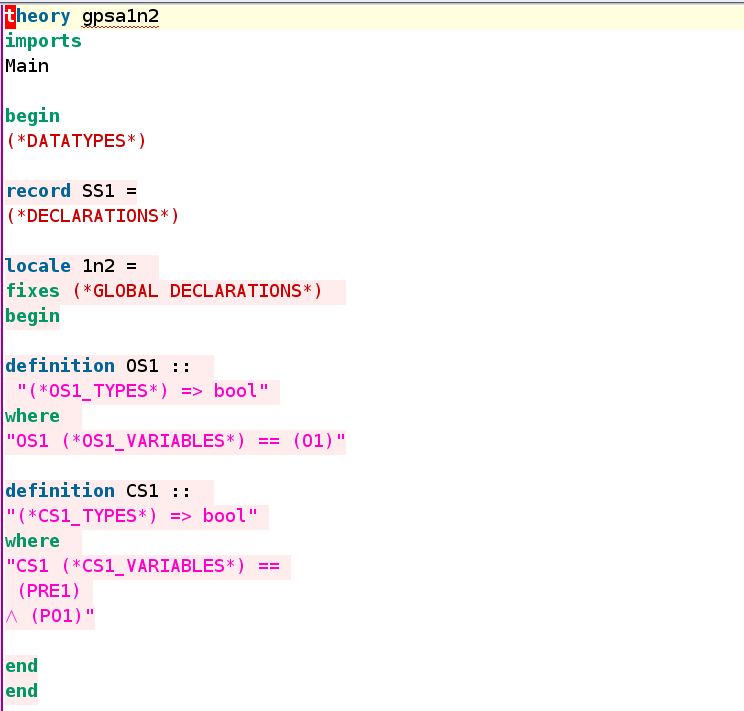
\includegraphics[clip, trim=0cm 0cm 15cm 0cm, scale=0.5]{examples/semiform/4image.png}
\vspace{-0.18in}
\caption{The Isabelle skeleton produced for the autopilot specification. \label{fig:autoisskel}}
\vspace{-0.2in}
\end{minipage}\hfill
\begin{minipage}{0.43\textwidth}
\centering
%[clip,l,b,r,t]
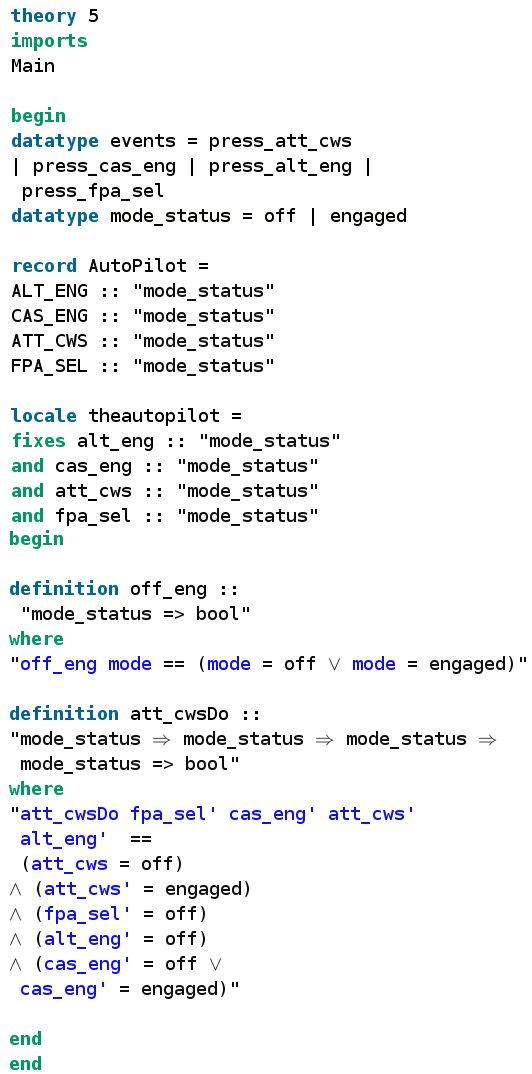
\includegraphics[clip, trim=0cm 0cm 4cm 0cm, scale=0.35]{examples/semiform/5imageal.png}
\vspace{-0.2in}
\caption{The autopilot specification in Isabelle syntax. \label{fig:autoisa}}
\vspace{-0.2in}
\end{minipage}
\end{figure}

\Gls{zmath} can automatically translate the \gls{gps} into Isabelle syntax
(figure \ref{fig:autoisskel}), this is now an Isabelle skeleton. The Isabelle
skeleton has not yet taken the \gls{zcga} information as one can get to this
step with just the \gls{zdra} annotated document. Once the Isabelle is filled in
(figure \ref{fig:autoisa}) we have the annotated specification in Isabelle form.
This can now give the user an idea of how to input their specification into
Isabelle syntax, without them having prior knowledge of Isabelle. It is
important to note that this is as far as the \gls{zmath} translation goes. Since
there are no state Invariants with this case study no lemma's to check for
consistency have been generated. The user can add the state Invariants in their
raw \LaTeX{} specification, or fully formalise their specification. Another way
to fully prove their specification is to add other properties to the Isabelle
document.



\section{Analysing examples}

In this section we analyse the examples we have successfully translated into
Isabelle and proved the sanity of the specification. 

We remind the reader of figure \ref{fig:timeline} in chapter \ref{ch:design}.
\Gls{zmath} is able assist the user with the translation of specification up to
the point where sanity properties are produced but not proven. In our largest
case study (section \ref{subsec:casestudy1}) the user did not have to look
through all the state changing schema's and write the sanity checks for all of
them. The properties were already generated for each changeSchema however, the
user did have to go through each property and prove it. In total, there were 21
changeSchema's and 1 set of stateInvariants, therefore there was 21 properties
which the user had to prove manually.


\subsection{ModuleReg}

The modulereg is one of our smallest examples, however with 1 set of
stateinvariants and 2 changeSchemas, \gls{zmath} automatically produces 2 lemma's
to check the sanity of the specification. An example of one of these lemmas is
shown in figure \ref{fig:modulereglemma1}. This is one of the lemma's
automatically generated and thus we have the `\emph{sorry}' command at the end
to show that it needs manual input from the user to complete the proof.

\begin{figure}[H]
\centering
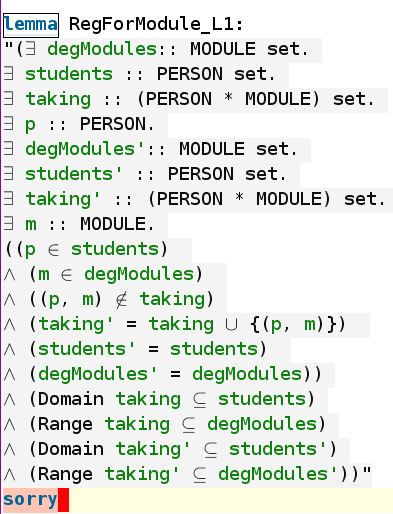
\includegraphics[scale=0.5]{Figures/Evaluation/lemmaformodulereg.png}
\caption{An example of one of the lemma's to check for consistency in the modulereg specification. \label{fig:modulereglemma1}}
\end{figure}

To prove this lemma we remove the `\emph{sorry}' command or put our curser at
the end of the lemma ready to input our methods to start the proof. In this case
`\emph{Auto sledgehammer}' again found a proof using the `\texttt{cvc4}'
\gls{smt} solver (shown in figure \ref{fig:autosolvermodulereg}). With this
lemma we are aiming to prove the sanity of the specification where the
changeSchema \verb|RegForModule| does not conflict with the stateInvariants
either before or after the state has been changed.

\begin{figure}[H]
\centering
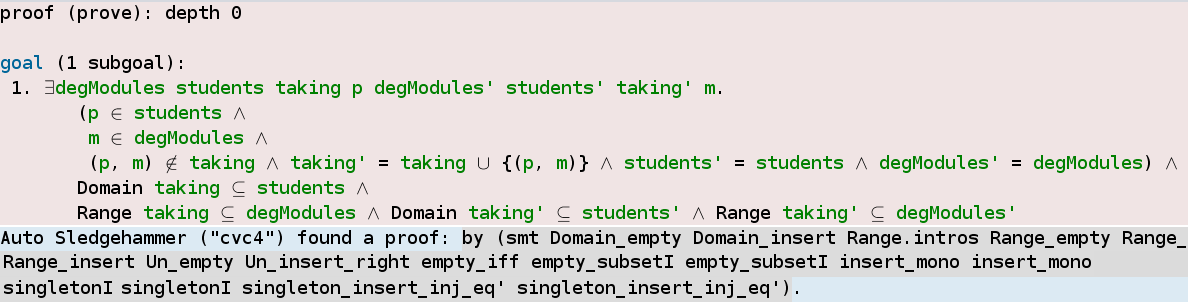
\includegraphics[scale=0.35]{Figures/Evaluation/moduleregproof.png}
\caption{Output shown when proving the lemma `\texttt{RegForModule} shown in figure \ref{fig:modulereglemma1} . \label{fig:autosolvermodulereg}}
\end{figure}

By clicking on the auto solving method shown in figure
\ref{fig:autosolvermodulereg} we can now complete the proof for the
\verb|RegForModule_L1| lemma. This is shown 

\begin{figure}[H]
\centering
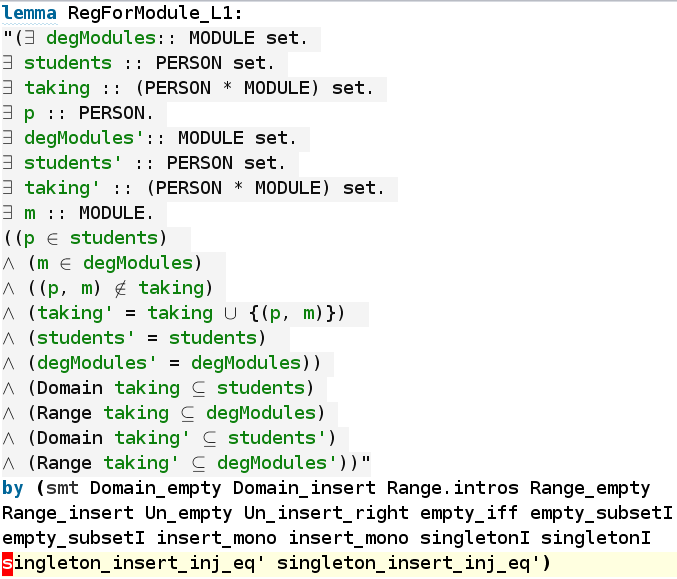
\includegraphics[scale=0.5]{Figures/Evaluation/provenmodulelemma.png}
\caption{The `\texttt{RegForModule}' lemma proved using Auto sledgehammer methods. \label{fig:solvedmodulelemma}}
\end{figure}

The second lemma in the moduleReg specification we managed to prove using
`\emph{blast}' thus having a complete proof for the complexity of the modulereg
specification.

We can see that the complexity of the proof used for the \verb|RegForModule_L1|
lemma in the modulereg specification is larger than the complexity of the proof
for the \verb|SNormalStop0_L1| in the steamboiler specification because it uses
more tactics.
There are other ways to measure
complexity of a proof (e.g. type of tactics used, time taken to prove etc). 
However for the purpose of this
thesis we say the more tactics we need to use for a proof the more complex it
is.  Although we
used `\emph{Auto sledgehammer}' to assist proving the lemma's there are 16
methods used in proving the \verb|RegForModule_L1| lemma (\verb|Domain_empty|,
\verb|Range_empty| etc.) compared with 1 method used in proving the
\verb|SNormalStop0_L1| lemma (\verb|State.distinct(9)|). Again we can say that
there might of been an alternate way to prove these particular lemma's however
we have chosen to prove them in this way to show variation. Since there are more
state changing schema's in the steamboiler specification there are also more
lemma's to prove with the steamboiler then there is in the modulereg
specification to obtain a fully proven specification which checks the complexity
of the system.

\subsection{Vending Machine}

The vending machine example has 3 state changing schemas (shown in table
\ref{tab:speczdracount}) however since it does not have any labeled
stateInvariants, \gls{zmath} can not automatically produce any properties to
prove the consistency of the specification. If we refer back to figure
\ref{fig:timeline} in chapter \ref{ch:design} it shows that the \gls{zmath}
tool-kit goes slightly past the point of `\emph{specification in isabelle with no
proof}' however the automation of \gls{zmath} can only go past that point
\textbf{if} there are changeschema's and stateInvariants labelled. Otherwise the
\gls{zmath} tool-kit can only translate the specification into isabelle syntax
with no lemma's or properties to prove. Thus it is up to the user to carry on
manually inputting their properties to obtain a fully proven specification.

\subsection{Other examples}

Each specification has a different amount of lemma's which the user needs to
prove depending on how many `stateInvariants' and `changeSchema's' there are. If
the specification does not have any stateInvariants then \gls{zmath} will not
produce any lemmas to prove for the sanity of the specification.

\begin{table}[H]
\begin{tabular}{|l | l | l |}
\hline
\textbf{Specification} & \textbf{Amount of} & \textbf{Total amount} \\
& \textbf{generated lemmas} & \textbf{of tactics} \\
\hline
Steamboiler & 20 & 41 \\
ProjectAlloc & 5 & 18 \\
VideoShop & 3 & 3 \\
TelephoneDirectory & 4 & 8 \\
ClubState & 4 & 4 \\
ZCGa & 6 & 6 \\
GenDB & 4 & 13 \\
Timetable & 4 & 4 \\
BirthdayBook & 1 & 1\\
AutoPilot & 0 & 0 \\
ClubState2 & 3 & 4 \\
Vending Machine & 0 & 0 \\
ModuleReg & 2 & 18 \\
\hline
\textbf{Total} & \textbf{56} & \textbf{120}\\
\hline
\end{tabular}
\caption{A table to show the amount of automatically generated lemmas and total amount of tactics used for each specification. \label{tab:lemmatact}}
\end{table}

We show the amount of lemmas and total amount of tactics needed to prove the
sanity of each specification in table \ref{tab:lemmatact}. Some lemma's need
only one tactic to be proved whilst other need a few. There are various
different ways to prove these lemmas and it all comes down to the personal
preference of the user. We have mainly used Isabelles `\emph{sledgehammer}' tool
to assist us with our proving.
We see that the AutoPilot specification has 0 generated lemmas and therefore 0
tactics to prove them. This is because the AutoPilot specification is only
semi-formalised and there will need to be \textit{preconditions}, \textit{changeSchemas} and
\textit{stateInvariants} to exist for the lemmas to be automatically generated.
Once the user adds these ZDRa categories to the Autopilot specification in a
formal manner (using Z) then the lemmas can be generated.

Proof complexity is a whole different research area that studies the concept of
complexity from the point of view of logic \cite{complexityofproofs}. It is connected with
computational complexity, but the goals are different. There are many ways to
measure `\textit{complexity} i.e. the size of the proofs, how strong theory is
needed to prove the theorem etc. Pudlak \cite{complexityofproofs} describes more on the
complexity of proofs. In order to discuss the complexity of proofs in this
thesis we will look at the size of the proof for each lemma.


% \subsubsection{SteamBoiler}

% The steamboiler has in total 20 lemmas to check the specifications sanity as it
% has 20 changing state schemas. The specification has 1 set of stateInvariants
% and we used 41 tactics to prove our lemmas.

% The steamboiler state invariants is shown in the expression part of the
% stateSchema. The state invariants for this specification is that the minimum
% water level (\verb|w_min|) must be smaller than the maximum water level
% (\verb|w_max|). Therefore, the state invariants are written after
% `\texttt{assumes}' in the specification (\verb|w_min < w_max|). 

% When \gls{zmath} produces the proof obligations to check the sanity of the
% specification it must also check that the changeSchema does not conflict with
% the prime state invariants. Thus, the proof obligations to check for all
% changing state schema will check that the preconditions and postconditions of
% each changeSchema still imply that (\verb|w_min < w_max|) \textbf{and}
% (\verb|w_min' < w_max'|).

% For example to prove our first lemma \verb|SNormalStop0_L1|, we wish to make
% sure that the \verb|SNormalStop0| changeSchema does not conflict with the
% stateInvariants and the stateInvariants prime.

% \noindent \begin{tabular}{|l | l|}
% \hline
% \verb|lemma (in  thesteamboiler)| & {\color{red}begin} \\
% \verb|SNormalStop0_L1:|& {\color{red}Name of lemma} \\
% \verb|"(\<exists> steamboiler0 :: | & \\
% \verb|SteamBoiler0.|&  {\color{red}list of all} \\
% \verb|\<exists> a' :: OnOff.|&  {\color{red}variables and} \\
% \verb|\<exists> steamboiler0' :: | & {\color{red}types} \\
% \verb|SteamBoiler0.|&  \\
% \verb|\<exists> w_max' :: nat.|&  \\
% \verb|\<exists> w_min' :: nat.|&  \\
% \verb|\<exists> z' :: State.|&  \\
% \verb|\<exists> v' :: OpenClosed.|&  \\
% \verb|(z = norm)|&  {\color{red}preconditions \textbf{and}}\\
% \verb|\<and> (w < w_min ∨|& {\color{red}postconditions of} \\
% \verb|w > w_max)|& {\color{red}SNormalStop0 schema} \\
% \verb|\<and> (a' = off \<and>|&  \\
% \verb|z' = stop)|&  \\
% \verb|\<longrightarrow> (w_min < w_max|& {\color{red}\textbf{implies}
% stateInvariants} \\
% \verb|\<and> (w_min' < w_max')))"|& {\color{red}\textbf{and} stateInvariants
% prime} \\
% \verb|by (smt State.distinct(9))|&  \\
% \hline
% \end{tabular}

% Since there are 2 records in our steamboiler specification we have to manually
% write the line \verb|(in the steamboiler)| which lets isabelle know that the
% changeSchema uses variables from the first record. The \verb|SNormalStop0_L1|
% lemma is proved using 2 tactics \verb|smt| and \verb|State.distinct(9)|. We
% remind the reader that although we have used these 2 tactics to prove our lemma
% there may be other ways in which to do so. 

% Our most complex proof is for the \verb|SNormalContinue1_L11| lemma in which we
%use 3 tactics to prove the property that the \verb|SNormalContinue1|
%changeSchema does not conflict with the state Invariants. The tactics we use
%here are \verb|smt|, \verb|OnOff.distinct(1)| and \verb|pswitch.simps(1)|.

\subsubsection{ProjectAlloc}

The projectAlloc specification \cite{mathlangexamples} has 5 changeSchema's and 1 set of stateInvariants
therefore it has 5 lemmas which \gls{zmath} has automatically generated to check
for the consistency. To prove these lemmas we have in total used 18 tactics.

The lemmas to check that the changeSchema's did not conflict with
the stateInvariants with were as follows:

\begin{verbatim}
\<exists> variables and types.
Preconditions
\<and>
PostConditions
\<longrightarrow>
(((dom studInterests) \<inter> (dom lecInterests) = {})
\<and> (dom allocation \<subseteq> dom studInterests)
\<and> (ran allocation \<subseteq> dom lecInterests)
\<and> (dom maxPlaces = dom lecInterests)
\<and>  (\<forall> lec \<in> dom maxPlaces.
(card ({l. the (allocation l) = lec})) \<leq> the (maxPlaces lec))
\<and>  ((dom studInterests') \<inter> (dom lecInterests') = {})
\<and> (dom allocation' \<subseteq> dom studInterests')
\<and> (ran allocation' \<subseteq> dom lecInterests')
\<and> (dom maxPlaces' = dom lecInterests')
\<and>  (\<forall> lec \<in> dom maxPlaces'.
(card ({l. the (allocation' l) = lec})) \<leq> the (maxPlaces' lec))))"
\end{verbatim}

Our most complex lemma to prove is the \verb|AddLecturer_L5| lemma which we used
9 tactics:

(\verb|metis|, \verb|full_types|, \verb|dom_empty|, \verb|dom_empty|,
\verb|dom_empty|, \\
 \verb|dom_eq_singleton_conv|, \verb|dom_restrict|,
\verb|inf.idem| and \verb|insert_not_empty|).

The most simple lemma to prove was \verb|AddStudent_L3| and \verb|DeAllocate_L2|
where we just used 1 tactic (\verb|fastforce| and \verb|auto| respectively).

%\begin{tabular}{|l l |} \hline \verb|lemma AddLecturer_L5:| & \\
%\verb|"(\<exists> projectalloc :: ProjectAlloc.| & \\
%\verb|\<exists> projectalloc' :: ProjectAlloc.| & \\
%\verb|\<exists> studInterests' :: (PERSON \<rightharpoonup> ((nat * TOPIC)
%set)).| & \\
%\verb|\<exists> lecInterests' :: (PERSON \<rightharpoonup> ((nat * TOPIC)
%set)).| & \\
%\verb|\<exists> allocation' :: (PERSON \<rightharpoonup> PERSON).| & \\
%\verb|\<exists> maxPlaces' :: (PERSON \<rightharpoonup> nat).| & \\
%\verb|\<exists> l :: PERSON.| & \\
%\verb|\<exists> maxAlloc :: nat.| & \\
%\verb|\<exists> ts :: ((nat * TOPIC) set).| & \\
%\verb|(l \<notin> ((dom studInterests) \<union> (dom lecInterests)))| & \\
%\verb|\<and> (lecInterests' = lecInterests(l \<mapsto> ts))| & \\
%\verb|\<and> (maxPlaces' = maxPlaces(l \<mapsto> maxAlloc))| & \\
%\verb|\<and> (studInterests' = studInterests)| & \\
%\verb|\<and> (allocation' = allocation)| & \\
%\verb|\<longrightarrow>(((dom studInterests) \<inter> (dom lecInterests) = {})|
%& \\
%\verb|\<and>(dom allocation \<subseteq> dom studInterests)| & \\
%\verb|\<and>(ran allocation \<subseteq> dom lecInterests)| & \\
%\verb|\<and>(dom maxPlaces = dom lecInterests)| & \\
%\verb|\<and> (\<forall> lec \<in> dom maxPlaces. (card ({l. the (allocation l)
%= lec})) \<leq> the (maxPlaces lec))| & \\
%\verb|∧ ((dom studInterests') \<inter> (dom lecInterests') = {})| & \\
%\verb|∧(dom allocation' \<subseteq> dom studInterests')| & \\
%\verb|∧(ran allocation' \<subseteq> dom lecInterests')| & \\
%\verb|∧(dom maxPlaces' = dom lecInterests')| & \\
%\verb|∧ (\<forall> lec \<in> dom maxPlaces'. (card ({l. the (allocation' l) =
%lec})) \<leq> the (maxPlaces' lec))))"| & \\
%\verb|by (metis (full_types) dom_empty dom_empty dom_empty| & \\
%\verb|dom_eq_singleton_conv dom_restrict inf.idem insert_not_empty)| & \\
%\end{tabular}

\subsubsection{VideoShop}

The videoShop specification \cite{mathlangexamples} has 3 changeSchemas and 1 set of stateInvariants,
therefore \gls{zmath} has generated 3 proof obligations to check that none of
the changeSchemas conflict with the stateInvariants and stateInvariants prime.

The structure of lemma's for the videoshop specification are as follows:

\begin{verbatim}
\<exists> variables and types.
Preconditions
\<and>
PostConditions
\<longrightarrow>
(Domain rented \<subseteq> members)
\<and> (Range rented \<subseteq> dom stockLevel)
\<and> (\<forall> t \<in> Range rented.
 card ({p. (p, t) \<in> rented}) < (the (stockLevel t)))
\<and> (Domain rented' \<subseteq> members')
\<and> (Range rented' \<subseteq> dom stockLevel')
\<and> (\<forall> t \<in> Range rented'.
 card ({p. (p, t) \<in> rented'}) < (the (stockLevel' t))))"
\end{verbatim}

We are able to prove all 3 lemma's by the tactic \verb|blast|. 

\subsubsection{TelephoneDirectory}

The telephone directory \ref{app:nonworkingzcga} has 1 set of stateInvariants and 4 changeSchema's.
Therefore we have 4 lemma's which \gls{zmath} generated and which we need to
prove. The structure for the lemmas to check the consistency of the telephone
directory specification are as follows:

\begin{verbatim}
\<exists> variables and types.
Preconditions
\<and>
PostConditions
\<longrightarrow>
((dom phoneNumbers = Domain persons)
\<and> (dom phoneNumbers' = Domain persons')))"
\end{verbatim}

These sanity check make sure that when updated the telephone directory that the
people listed in the domain of phoneNumbers is equal to the list in the domain
of persons.

To prove the first 2 lemmas \verb|AddPerson_L1| and \verb|RemoveNumber_L2| we
only needed to use a single tactic (\verb|auto| and \verb|fastforce|)
respectively. However the last 2 lemmas (\verb|RemovePerson_L3| and
\verb|RemoveNumber_L4|) required 3 tactics each. For example to prove the
\verb|RemovePerson_L3| lemma we needed to use \verb|smt|,
\verb|Diff_insert_absorb| and \verb|mk_disjoint_insert|. In total we used 8
tactics to prove all 4 properties.

\subsubsection{ClubState}

The clubstate specification \cite{mathlangexamples} has 4 changing schemas and thus 4 properties to
check the state invariants are not conflicted when the state has been changed.
The stateinvariants for the clubstate specification is are as follows:

\begin{verbatim}
\<exists> variables and types.
Preconditions
\<and>
PostConditions
\<longrightarrow>
(hall \<subseteq> badminton) 
\<and> (card hall \<leq> maxPlayers)
\<and> (hall' \<subseteq> badminton') 
\<and> (card hall' \<leq> maxPlayers))"
\end{verbatim}

Here we wish that all the people in the hall must be members of badminton and
the number of players can not exceed the maximum amount both before the change
and after the change in state. The first 2 lemma's in our clubstate
specification (\verb|LeaveHall_L1| and \verb|AddMember_L2|) were proven by
\verb|auto| and the last two properties (\verb|EnterHall_L3:| and
\verb|RemoveMember_L4|) were proven by \verb|blast|.

\subsubsection{ZCGa}

In the specification \cite{mathlangexamples} representing the \gls{zcga} we have 6 properties to prove.
The syntax for the properties which \gls{zmath} has generated are:

\begin{verbatim}
\<exists> variables and types.
Preconditions
\<and>
PostConditions
\<longrightarrow>
(TermDeclaration \<subseteq> declarations)
\<and> (SetDeclaration \<subseteq> declarations)
\<and> (dvars \<subset> sets \<union> terms)
\<and> (sets \<inter> terms = {})
\<and> (TermDeclaration' \<subseteq> declarations')
\<and> (SetDeclaration' \<subseteq> declarations')
\<and> (dvars' \<subset> sets' \<union> terms')
\<and> (sets' \<inter> terms' = {}))"
\end{verbatim}

Since we have 6 changing schemas we need to check that none of the schemas
conflict with the stateInvariants before and after the state has been changed.
In this proof, we have proven 2 lemmas

(\verb|CorrectExpression_L1| and \verb|CorrectConstantTerm_L5|) by \verb|smt|
and the remaining 4 using \verb|blast|.

\subsubsection{GenDB}

GenDB \cite{mathlangexamples} has 4 consistency checks we must prove against the stateInvariants. The
syntax for the stateInvariants are as follows:

\begin{verbatim}
\<exists> variables and types.
Preconditions
\<and>
PostConditions
\<longrightarrow>
(Domain parent \<union> Range parent \<subseteq> dom sex
\<and> (\<forall>p :: PERSON. (p, p) \<notin> parent^*)
\<and> (\<forall>p :: PERSON. \<forall>q :: PERSON.
\<forall>r :: PERSON. ({(p,q),(p,r)} \<subseteq> parent)
\<and> q \<noteq> r \<longrightarrow>
the (sex q) \<noteq> the (sex r)))
\<and> (Domain parent' \<union> Range parent' \<subseteq> dom sex'
\<and> (\<forall>p :: PERSON. (p, p) \<notin> parent'^*)
\<and> (\<forall>p :: PERSON. \<forall>p :: PERSON.
\<forall>r :: PERSON. ({(p,q),(p,r)} \<subseteq> parent')
\<and> q \<noteq> r \<longrightarrow>
the (sex' q) \<noteq> the (sex' r))))"
\end{verbatim}

Out of the 4 lemmas we proved, 2 lemmas can be proven by the tactic \verb|blast|.
The other 2 lemmas we proved by using 5 other tactics. For example, we proved the
\verb|AddPerson_L3| property using the tactics \verb|metis|, \verb|mono_tags|,
\verb|lifting|, \verb|empty_iff| and \verb|rtrancl.rtrancl_refl|. This made sure
that when a person has been added to the genDB that the preconditions and
postconditions satisfied the stateInvariants.

\subsubsection{Timetable}

The timetable specification \cite{mathlangexamples} has 4 schemas in which the original state has
changed and 1 set of stateInvariants that must be obeyed throughout the
specification. The stateInvariants for the timetable specification are as
follows.

\begin{verbatim}
\<exists> variables and types.
Preconditions
\<and>
PostConditions
\<longrightarrow>
(\<forall> s \<in> dom studentTT. \<forall> m \<in> dom moduleTT.
(the (studentTT s) \<inter> the (moduleTT m) \<noteq> empty)
\<longrightarrow>
(dom (the (studentTT s))) moduleTT m = (dom (the (studentTT s)))))
\<and> (\<forall> s \<in> dom studentTT'.
 \<forall> m \<in> dom moduleTT'.
(the (studentTT' s) \<inter> the (moduleTT' m) \<noteq> empty)
\<longrightarrow>
(dom (the (studentTT' s))) moduleTT' m = (dom (the (studentTT' s))))"
\end{verbatim}

There are 4 properties to prove in the timetable specification. We have been
able to prove 3 properties (\verb|RegForModule_L1|, \verb|AddStudent_L2| and
\verb|ScheduleModule_L4|) using \verb|smt| and 1 property
\verb|DescheduleModule_L3| using \verb|blast|.

\subsubsection{BirthdayBook}

Since we used the simplest form of the birthdaybook \ref{app:bb} specification (there are
many different forms) we only had 1 lemma to prove. The \verb|AddBirthday_L1|
property was proven by \verb|auto| however we could have also solved it using
\verb|smt|.

\begin{verbatim}
\<exists> variables and types.
Preconditions
\<and>
PostConditions
\<longrightarrow>
(known = dom birthday)
\<and> (known' = dom birthday'))"
\end{verbatim}

\subsubsection{ClubState2}

The clubstate2 specification \cite{mathlangexamples} is an extension of the original clubstate
specification. Since the specification stemmed from the original clubstate we
have to make sure that the changeState schemas do not conflict with the
stateInvariants from the first stateSchema as well as the stateInvariants in the
ClubState2 state schema. We have the following stateInvariants from the
ClubState2 specification:

\begin{verbatim}
\<exists> variables and types.
Preconditions
\<and>
PostConditions
\<longrightarrow>
((hall \<subseteq> badminton)
\<and> (card hall \<leq> maxPlayers)
\<and> [onCourt, (Range waiting)] partition [hall]
\<and> (hall' \<subseteq> badminton')
\<and> (card hall' \<leq> maxPlayers)))
\<and> [onCourt', (Range waiting')] partition [hall']"
\end{verbatim}

The stateInvariants taken from the ClubState2 state schema is

 \verb|[onCourt, (Range waiting)] partition [hall]| however the ClubState2 state
 schema uses the ClubState schema. Therefore the original stateInvariants

(\verb|((hall \<subseteq> badminton)| and \verb|(card hall \<leq> maxPlayers)|)
must also be checked.

The 3 lemmas which needed to be proved use a total of 4 tactics. The first and
last lemmas are proven by \verb|auto| where as the second lemma
(\verb|LeaveHall_L2|) is proven using 2 tactics (\verb|smt| and
\verb|empty_iff|).

\subsubsection{ModuleReg}

The ModuleReg specification has 2 changeSchemas and 1 set of stateInvariants.
therefore \gls{zmath} has produced 2 lemmas which we need to prove.

\begin{verbatim}
\<exists> variables and types.
Preconditions
\<and>
PostConditions
\<longrightarrow>
 (Domain taking \<subseteq> students)
\<and> (Range taking \<subseteq> degModules)
\<and> (Domain taking' \<subseteq> students')
\<and> (Range taking' \<subseteq> degModules'))"
\end{verbatim}

The \verb|AddStudent_L2| property we managed to prove using a single tactic
(\verb|blast|) however to prove the first lemma (\verb|RegForModule_L1|) we used
17 tactics, these were:

\begin{verbatim}
smt Domain_empty Domain_insert Range.intros Range_empty 
Range_insert Un_empty Un_insert_right empty_iff empty_subsetI 
empty_subsetI insert_mono insert_mono singletonI singletonI 
singleton_insert_inj_eq' singleton_insert_inj_eq'
\end{verbatim}

\subsection{Summary}
In conclusion we can see our examples how each of the lemma's are proven in
order to check the sanity of the specification. The amount of tactics used in
the specification does not depend on the amount of lemma's generated. The
complexity of the lemma can be measured in a variety of different ways
\cite{complexityofproofs} and therefore some specification will require more or
less strategies to prove (or more complex strategies). For example the Module
Reg specification has 2 lemmas but requires 18 tactics to be proved. Whereas the
Timetable specification has double the amount of lemma's (4) and only requires 4
tactics to prove the specification. Therefore the complexity of the
specification can not be measured in terms of "number of lemmas".
Finding proofs for these lemma's has to be done manually (or using the automated
help already in Isabelle). Some specification will require more theorem prover
expertise (moduleReg) in order to complete the final step to have a fully proven
specification. Whereas others (Timetable) will require less theorem prover
expertise to prove  the automatically generated lemmas. Therefore the amount of effort for
the last step of ZMathlang is difficult to measure as it depends on the
specification to be proven.


\section{Reflection and Discussion}

To check the consistency (section \ref{sec:proofobl}) of all our specification we had to prove 56 lemmas with
a total of 120 tactics. In this section we discuss how far the \gls{zmath}
tool-kit can take us,how difficult it is for the user to get the full proof and
what other proof is left.

\subsection{How far can ZMathLang tool-kit take us and what is left for the user to do manually.}

Looking back at our examples described in the previous section. The more
complex the language of the specification (whether it uses terms and set or just
terms), the more complex the proofs and syntax of the proofs are. The vending
machine has no stateinvariants therefore \gls{zmath} does not generate any
lemmas to be proven. This does not mean that stateInvariants are good or bad, it
means that the ZMathLang toolkit will be unable to generate any lemma to check
for the  consistency of the specification without them. The steamboiler specification, which is our longest
example, uses only terms but has 2 stateSchemas and therefore 2 records. We were
able to prove all the lemmas using 2 different automatic isabelle tools (blast
and sledgehammer).

We remind the reader of figure \ref{fig:timeline} in chapter \ref{ch:design},
\verb|sledgehammer| and \verb|blast| are the two tools which have the most
automated proving power. With the manual proof to complete the theorem the user
should have some basic knowledge of how to prove lemmas in Isabelle, at least
have some basic knowledge of the Isabelle tools available to assist them in
proving the lemmas. If the software/system designer is not an Isabelle expert
and has got up to step 5 in the \gls{zmath} steps then they would have the three
following options:

\begin{enumerate}
\item Learn no Isabelle at all and pass on the proofs to be completed by an
Isabelle expert.

\item Learn Isabelle in depth until they gain enough knowledge to prove their
specification and add more proofs if needed.

\item Learn the basic automated proving tools (highlighted in figure
\ref{fig:timeline}) to prove all (if not then some) of the lemmas, then hand the
rest to an Isabelle expert to finish off.
\end{enumerate}

In the first case we will need 2 people to complete the proof. Since the system
designer has already translated the specification into Isabelle syntax
automatically so a lot of the work has been done. The theory file has been set
up and properties have been written, the expert will just need to prove them.
Therefore a big chunk of work has been done. With this approach the majority of
the work goes 
to the system designer as they do not need to learn anything beyond their
existing knowledge. However, there
needs to be an Isabelle expert ready to complete the proofs and depending on the
syntax of the specification this may be difficult to prove. There also might be
other properties which the stakeholders of the project may wish to be proven.
Again, to add these extra properties, a little bit more Isabelle knowledge is
needed.

In the second scenario we will need only 1 person to complete the proof (the
system designer). Using the \gls{zmath} tool-kit will assist the designer
translating the specification into Isabelle syntax, however the user will then
need to learn more Isabelle to finish of the proof for their specification.
Since the \gls{zmath} has already produced an Isabelle file the user can then
learn the Isabelle syntax by example as well as reading through the various
Isabelle documentations online. In this scenario 
there is only one person doing the entire proof, there is less cost in finding
another Isabelle expert and paying them to complete the proof (depending on
the specification). The system engineer has to spend more time on learning
Isabelle syntax and proving in Isabelle which may become long and tedious. The
stakeholders may also want other properties proven about the specification which
again is down to the system designer to learn.

The third case is a compromise between the first two scenarios, it will require
the system designer and on some occasions and an Isabelle expert. The system
engineer translates the specification into Isabelle using the \gls{zmath}
tool-kit to assist them. They then learn the very basic automated proving tools,
to assist them in proving the lemmas to check for consistency. By doing this the
system engineer may be able to prove the entire specification for consistency
using the automated tool. However some lemmas if they are more complex may
require more Isabelle skills then just the automated Isabelle tools to prove.
Therefore the system engineer will be required to prove as much as they can and
if there are some parts which can not be proved with automation, they can pass
this along to an Isabelle expert. The Isabelle expert will then have less work
to prove the remainder of the proof. If the stakeholders require more properties
proved then the Isabelle expert can do this as well.

In the third cas an Isabelle expert may not be
required and proving the specification \textit{could} be done by one person
(depending on the specification) if the stakeholders only want to check the system for consistency
and
the syntax of the specification is relatively easy where automated tools can be
used to prove the specification. However, depending on the complexity of the
specification, an Isabelle expert may be needed sometimes if the system designer
can not prove the entire specification with just the automated tools and/or if
the stakeholders require a more rigorous proof.

Automation on both sides are constantly being redeveloped and revisited. One can
automate a specification into Isabelle covering formal methods and perhaps one
day, informal specification could be translated. On the other end, there are
many \gls{smt} solvers being develop to cover more and more existing lemmas and
theorems. However, due to the variations in systems, syntax and properties the
user may wish to prove, it is difficult to cover everything. The more complex
the system, the less automation available to assist in the users proofs. For a
simple system, there exists automation on both sides to cover the proofs.
However, once the user wishes to build a more complex system, the user will then
need to learn more about their chosen theorem in order to check for complete
correctness.

\subsection{Assumptions and limitations of the ZMathLang tool-kit}

The recommendations made in this thesis are based on several assumptions and
limitations as to what may be done to translate a Z specification into Isabelle
using our \gls{zmath} tool-kit.

The assumptions are as follows:

\begin{itemize}
\item Firstly, we like to point out that the \gls{zmath} can only translate
specifications with syntax used in our examples. Since the language of
mathematical notation is vast we can not incorporate the entire syntax of
mathematics in the \gls{zmath} within the scope of this thesis. More explanation
is given on this topic in the next chapter.

\item The \gls{zmath} tool-kit uses \LaTeX{} and is implemented in 
\verb|python2.7|. It uses the following python packages:
\begin{itemize}
\item \textbf{re:} To read the users annotations from \gls{zcga} and \gls{zdra}.
\item \textbf{networkx:} To implemented the instances and relationships into a
graph form.
\item \textbf{matplotlib:} To produce the goto and dependency graphs.
\item \textbf{Tkinter:} To run the user interface.
\end{itemize}

We assume that a user wanting to use the \gls{zmath} tool-kit has installed the
correct packages.

\item One of the assumptions the tool-kit makes is that if the specification
holds 1 state schema (and thus 1 record) then all the lemma's produced are under
that record. Thus, if the specification holds 2 or more records then the lemmas
produced will need to define which record they belong to. For example in the
SteamBoiler specification we manually input `\verb|(in thesteamboiler)|' after
the word `\verb|lemma|'. This does not have to be done to specification which
only hold one state schema.

\item Another assumption the \gls{zmath} tool-kit makes is that the document it is
checking contains a single specification. Although the \gls{zcga} can check
multiple specification in a single document, the rest of the tools assume that
it is checking 1 system. Thus, when producing the dependency and goto graphs and
the specification isn't linked, it will assume that the instances are under one
specification. Also when the \gls{zdra} translates the specification into
Isabelle it will do so in a single theorem document. More discussion on this is
in the `Future work' section in the next chapter.

\item We also assume that the user actually wishes to check the specification
for consistency. As Stepney discussed in \cite{stepney1998tale} there are many
properties to prove in a system. It is down to the stakeholders and clients of
the project. For example a high integrity system may have some universal
guidelines or codes of conduct it must obey. Proving properties to check for
consistency is highly valuable, however other properties such as if
preconditions hold, or relationship between two specification may also be wanted
by the project stakeholders. These other properties may be added at the end of
stage 6 and if the consistency checks are not needed, they can be deleted from
the Isabelle file manually.

\end{itemize}

We like to highlight the limitations of the \gls{zmath} tool-kit. They are as
follows:

\begin{itemize}
\item One of the limitations of the \gls{zmath} tool-kit is in the way the
\gls{zdra} checks if the specification is correctly totalised. Although an
incorrectly totalised specification can still be translated into Isabelle a
warning message comes up for incorrectly totalised specifications. If the users
totalises preconditions e.g \verb|\totalises{TS#}{PRE#}| and all preconditions
have been totalised then no warning appears. However, if the user totalises
schemas which hold preconditions within them e.g. \verb|\totalises{TS#}{CS#}|
then the \gls{zdra} checker doesnt pick up on it and would say the specification
is incorrectly totalised.

\item Another limitation is in the way the dependency and goto graphs are
presented. If the specification is relatively small, with not a lot of instances
and connections then the graphs a presented quite clearly. On the other hand,
when a specification is more complex with many instances the graph presents the
nodes bundled together. Visually this becomes difficult to see the relationship
between the nodes, it would be better if the nodes were represented with larger
spaces between them.
\end{itemize}

\section{Expert Reviews}

We gave experts from various fields and industries an overview of the \gls{math}
framework and asked for their opinion on it. The following questions were asked:

\begin{enumerate}
    \item Would you use ZMathLang toolkit for any of your work?
    \item Do you see the ZMathLang toolkit being useful somewhere in your work? If yes where and what steps in particular?
    \item Is breaking yo the translation path easier/harder/same with ZMathLang toolkit and why?
    \item Any other comments.
\end{enumerate}

The responses we got from the various industry expert were the following:\\
\noindent\fbox{%
\parbox{\textwidth}{%
\textit{The first two steps of ZMathLang would be useful in ordering the requirements 
in a logical order, this would greatly help the customer. The specificications
we write are for systems which have a quick turnaround therefore we don't 
usually do proofs on our specifications as it is too expensive both in
manpower and costs so the last steps would be redundant.} \\
\textbf{Bid Manager @ QinetiQ}}}\\

\noindent\fbox{%
\parbox{\textwidth}{%
\textit{As a Bid Solution Architect working in the Aerospace and Defence domain handling
a multitude of requirements can be a highly complex, especially when developing 
solutions and concepts that comprise of systems of systems. Steps 0 to 3 of
ZMathLang would facilitate the ordering of specific requirements quickly and 
effectively. Furthermore, the dependency graph is extremely useful for tracking
changes of a solution, whereby it would enable System Engineers to easily
identify the significance of a proposed change and the knock-on implications,
thus allowing for more expedient and accurate cost estimating.
If ZMathLang can be deployed easily with short user implementation time,
steps 0 to 3 would be beneficial throughout complex programmes.} \\
\textbf{Bid Solution Architect @ Thales}}}\\

\noindent\fbox{%
\parbox{\textwidth}{%
\textit{The ZMathLang Toolkit
appears to be an useful program. However at the moment all controller 
specifications are written by engineers and then checked and approved by 
two other senior/principal engineers. There is no room for language and logical errors. 
I see the subjected toolkit useful when autonomous vehicles would be 
introduced on our roads. New, more complicated programs and controller 
specifications would be expected to be developed to assure an appropriate
connection is kept between vehicles approaching to the 
junctions/pedestrian crossings and controllers.  
The ZMathLang could then be used to assist users to analyse and highlight 
any logical and language errors, inconsistencies and mistakes especially if 
the new controller specifications/other programs would require more then 
one person working on it especially from different teams.} \\
\textbf{Traffic Signal Engineer @ AECOM}}}\\
\\
\noindent\fbox{%
\parbox{\textwidth}{%
\textit{Aviation engineering encompasses a large range of disciplines where the ZMathLang
toolkit would provide assistance to work carried out by both myself and colleagues
at conceptual and detailed stages of design. 
A few examples of where the toolkit could be used are as follows; 
Conceptual design of airfields entails a series of well organised requirements from
clients with processes enabling designers to make logical and objective decisions. 
Steps 0-2 of the toolkit would be particularly useful within this work. 
However design does, to a certain degree, require human interference in the process. 
The ZMathLang toolkit could provide useful automation to the surface 
access issues within an airfield masterplan. This would include the 
automation of passenger buses from airport terminal to aircraft stands. 
All steps within the toolkit would provide a complete analysis and successful
implementation. Whilst as an aviation engineer working on airfield design specifically, 
I believe the toolkit would have further benefits to the wider aviation industry. 
Further automation in the industry is sought as technology is continuously improving. 
I would consider the toolkit could play an important part in the improvement of baggage 
handling systems, discussions around the automation of air traffic control services, 
and an airline's approach to their operations with regards to aircraft movements and 
the associated efficiencies.} \\
\textbf{Aviation Engineer @ AECOM}}}\\

Overall the feedback we receive on the \gls{zmath} was quite positive especially
for the first steps of the toolkit. Three out of the four reviews highlighted
that the \gls{zcga} and \gls{zdra} would be the most useful in their domain of
work. One of the reviews specifically mentioned that in a fast line of work
where systems need to be delivered to the customer quickly it is rare for them
to create proofs for their specification (system engineer review), whereas
another review mentioned that the entire toolset would be useful (traffic signal
engineer). In summery, the comments given by various industry professionals seem
to indicate that the \gls{zmath} toolkit would be useful especially the first
two steps (\gls{zcga}, \gls{zdra} and the dependency graphs). However these
comments where given by reading an overview of the \gls{zmath} toolkit (except
for the system engineer review where \gls{zmath} was physically demonstrated).

\section{Conclusion}

The \gls{zmath} tool-kit has been tried and tested on various examples of Z
specifications. We have translated specifications with syntax using set and
terms and specifications using terms only. It seems that the grammatical types
do not affect the ease of translation, but the amount of instances and the
notations of mathematics do. The Steamboiler specification was our most complex
example and we had to manually input extra parts to the lemmas in order to prove
them. The amount of changeSchema's and stateInvariants affect how many
properties the tool-kit will produce. The complexity of the mathematical notation
will determine how difficult the properties are to prove, whether they can be
proven with the assistance of automatic tools or whether they need more Isabelle
expertise to prove. Expert reviews on the \gls{zmath} toolkit conclude that
toolset could be useful in various domains.

We have outlined some of the assumptions and limitation of the \gls{zmath}
tool-kit and we discuss the achievements of the system and future work in the next
chapter.
